\documentclass[twoside,english]{article}
\setlength{\oddsidemargin}{0.25 in}
\setlength{\evensidemargin}{-0.25 in}
\setlength{\topmargin}{-0.6 in}
\setlength{\textwidth}{6.5 in}
\setlength{\textheight}{8.5 in}
\setlength{\headsep}{0.75 in}
\setlength{\parindent}{0 in}
\setlength{\parskip}{0.1 in}

\usepackage{amsmath,amsfonts,graphicx,algorithm,caption}
\usepackage[noend]{algpseudocode}
\usepackage[numbers]{natbib}
\usepackage{hyperref}
\usepackage[document]{ragged2e}
\usepackage{mathtools}
\usepackage{xcolor}
\usepackage{booktabs}
\usepackage{multirow}
\usepackage{listings}
\usepackage{url}

\lstset{
  basicstyle=\ttfamily\small,
  breaklines=true,
  frame=single,
  backgroundcolor=\color[gray]{0.96},
  columns=fullflexible,
  keepspaces=true,
}

\newcounter{lecnum}
\renewcommand{\thepage}{\arabic{page}}
\renewcommand{\thesection}{\arabic{section}}
\renewcommand{\theequation}{\arabic{equation}}
\renewcommand{\thefigure}{\arabic{figure}}
\renewcommand{\thetable}{\arabic{table}}
\makeatletter
\def\BState{\State\hskip-\ALG@thistlm}
\makeatother

\newcommand{\lecture}[4]{
   \pagestyle{myheadings}
   \thispagestyle{plain}
   \newpage
   \setcounter{page}{1}
   \noindent
   \begin{center}
   \framebox{
      \vbox{\vspace{2mm}
    \hbox to 6.28in { {\bf IE 663: Advanced Topics in Deep Learning
		\hfill Jan-April 2026} }
       \vspace{4mm}
       \hbox to 6.28in { {\Large \hfill Project Report: #1  \hfill} }
       \vspace{2mm}
       \vspace{2mm}
       \hbox to 6.28in { {\it Team Name: #2 \hfill Team Members: #3} }
      \vspace{2mm}}
   }
   \end{center}
   \vspace*{4mm}
}

\newcommand{\fig}[3]{
			\vspace{#2}
			\begin{center}
			Figure #1:~#3
			\end{center}
	}

\newtheorem{theorem}{Theorem}[lecnum]
\newtheorem{lemma}[theorem]{Lemma}
\newtheorem{proposition}[theorem]{Proposition}
\newtheorem{claim}[theorem]{Claim}
\newtheorem{corollary}[theorem]{Corollary}
\newtheorem{definition}[theorem]{Definition}
\newenvironment{proof}{{\bf Proof:}}{\hfill\rule{2mm}{2mm}}

\newcommand{\R}{\mathbb{R}}

\begin{document}

\lecture{Task-Subspace Logit Attribution}{$<>$}{23B0932}

% ============================================================================
% ABSTRACT
% ============================================================================
\begin{abstract}
Large language models can learn new tasks from just a few examples placed in their input prompt, a capability known as in-context learning (ICL). But \textit{how} this works internally remains poorly understood. Recent mechanistic interpretability work proposes that ICL decomposes into two separable sub-computations carried out by distinct attention heads: \textbf{task recognition} (TR), which identifies what task is being performed, and \textbf{task learning} (TL), which maps the specific input to the correct output. We reproduce and extend the core experiments from \cite{TSLA} on SST-2 sentiment classification using an 8-shot ICL setup with \texttt{unsloth/Llama-3.2-3B-Instruct-bnb-4bit}, a 4-bit NF4 quantized Hugging Face checkpoint derived from Meta's Llama-3.2-3B-Instruct. Across five experiments, viz.\ head identification, overlap analysis, ablation, layer-wise distribution, and attention allocation, we find that TR heads are mechanistically closer to induction heads than TL heads are, that TR heads concentrate in deeper layers, and that TR and TL heads attend to structurally different parts of the prompt. These results qualitatively align with the original paper, supporting the hypothesis that task recognition and task learning are distinct computations localized to different attention heads.
\end{abstract}

% ============================================================================
% 1. INTRODUCTION
% ============================================================================
\section{Introduction} \label{sec:intro}

In-context learning is one of the most striking emergent abilities of large language models. Without any gradient updates, a model can be prompted with a handful of input-output examples and reliably generalize to a new query, performing sentiment analysis, translation, or arithmetic purely from the pattern in its context window. This raises a natural question: what internal mechanisms enable this?

Mechanistic interpretability offers a way to answer this by opening the model and studying the roles of individual components, particularly attention heads. The key insight motivating this project is that ICL might not be a single monolithic computation. Instead, it may decompose into two phases: first, the model figures out \textit{what task} is being demonstrated (task recognition), and then it applies the learned mapping to \textit{produce the answer} for the query (task learning).

This separation was formalized by \cite{TSLA}, who introduced quantitative scores to classify attention heads as TR or TL heads, and showed that these head sets are largely disjoint, occupy different layers, and have different ablation signatures. Our project reproduces this analysis on a smaller model and a single dataset (SST-2) to test whether the core findings hold in a scaled-down setting.

% ============================================================================
% 2. WORKFLOW
% ============================================================================
\section{Project Workflow} \label{sec:workflow}

\begin{enumerate}
    \item \textbf{Paper reading and conceptual grounding.} Read the primary paper \cite{TSLA} along with foundational work on transformer circuits \cite{TransformerCircuits} and induction heads \cite{InductionHeads}. Built intuition for the residual stream, unembedding, and the role of attention heads.
    \item \textbf{Scope definition.} Chose SST-2 as the single task and \texttt{unsloth/Llama-3.2-3B-Instruct-bnb-4bit} as the model, given Kaggle GPU constraints.
    \item \textbf{Codebase development.} Implemented modular Python source files for prompt construction, token bookkeeping, attention/value extraction, TR/TL/IH scoring, ablation, and plotting.
    \item \textbf{Experiment execution.} Ran all five experiments on Kaggle (P100 GPU, 16 GB VRAM).
    \item \textbf{Analysis and report writing.} Interpreted results, compared against paper expectations, and wrote this report.
\end{enumerate}

% ============================================================================
% 3. BACKGROUND AND INTUITION
% ============================================================================
\section{Background and Intuition} \label{sec:background}

\subsection{The Residual Stream}

A transformer processes a sequence of tokens by passing them through a stack of layers. At each layer, the attention mechanism and the MLP read from a running sum called the \textit{residual stream} and write their outputs back into it. The final token representation is just the sum of the original embedding plus every layer's contribution. This additive structure is key: it means each attention head's output is a vector that gets added directly to the residual stream, and we can study heads independently by looking at what each one contributes.

\begin{figure}[h!]
    \centering
    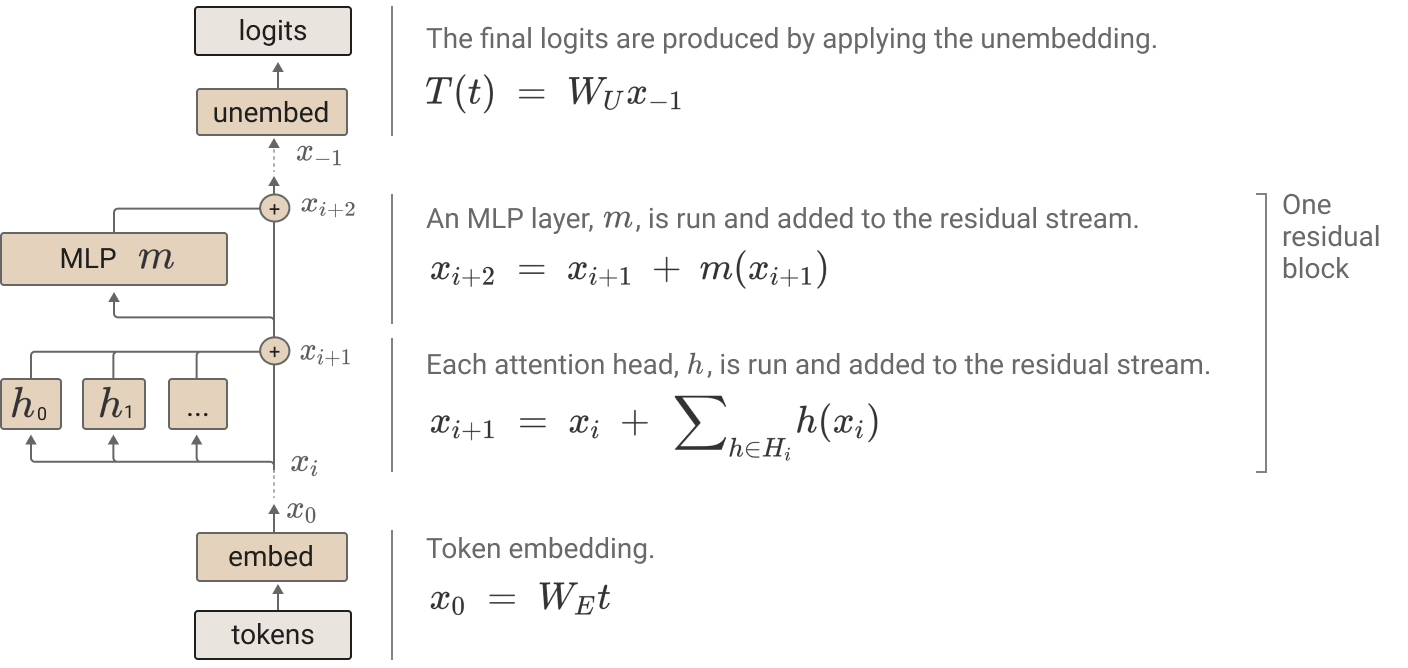
\includegraphics[width=0.75\linewidth]{assets/transformer-model.png}
    \caption{Schematic of a transformer layer showing the residual stream and attention head contributions. Each head's output is a vector added to the residual stream, which is why we can analyze heads in isolation.}
    \label{fig:transformer-model}
\end{figure}

Concretely, the residual stream at the final token position after all $L$ layers can be written as:
\begin{equation}
x_{\text{final}} = x_{\text{emb}} + \sum_{l=1}^{L} \left( \sum_{k=1}^{H} a_{l,k} + m_l \right)
\end{equation}
where $x_{\text{emb}}$ is the token embedding, $a_{l,k}$ is the output of attention head $k$ at layer $l$, and $m_l$ is the MLP output at layer $l$. The logits are then $z = W_U \, x_{\text{final}}$. Substituting, the logit for any vocabulary token $v$ decomposes as:
\begin{equation}
z_v = w_v^\top x_{\text{emb}} + \sum_{l,k} w_v^\top a_{l,k} + \sum_l w_v^\top m_l
\end{equation}
where $w_v$ is the $v$-th row of $W_U$. The term $w_v^\top a_{l,k}$ is the \textit{direct logit contribution} of head $(l,k)$ to token $v$. This is the quantity that makes per-head attribution possible: each head's influence on the final prediction is just an inner product between its output vector and the unembedding direction of interest.

A useful analogy is to think of the residual stream as a shared communication bus with fixed bandwidth. The hidden dimension $d$ determines the total number of independent ``channels'' available for heads to pass information through. Each attention head does not get to write to the entire $d$-dimensional space equally; instead, each head projects its output into a low-rank subspace of dimension $d_h = d / H$ (where $H$ is the number of heads). In our model, this is $128 = 3072 / 24$. So each head effectively ``owns'' a 128-dimensional slice of the full 3072-dimensional stream. The output projection $W_O$ then maps these per-head subspaces back into the full residual stream, but the key point remains: each head's contribution is a low-rank update, and different heads can write to largely independent subspaces without interfering with each other.

To make this precise, consider head $k$ at layer $l$. It computes a $d_h$-dimensional vector $h_{l,k} \in \R^{d_h}$ from the attention-weighted value states. This vector is then mapped back to the full residual stream by the output projection:
\begin{equation}
a_{l,k} = W_O^{(k)} \, h_{l,k}
\end{equation}
where $W_O^{(k)} \in \R^{d \times d_h}$ is the slice of the output projection matrix corresponding to head $k$. Because $d_h \ll d$, the output $a_{l,k}$ lives in (at most) a $d_h$-dimensional subspace of $\R^d$, namely the column space of $W_O^{(k)}$. The columns of $W_O^{(k)}$ form a basis for the ``writing subspace'' of head $k$: the set of directions in the residual stream that this head can influence. No matter what input the head receives, its contribution to the residual stream is confined to $\operatorname{col}(W_O^{(k)})$.

\begin{figure}[h!]
    \centering
    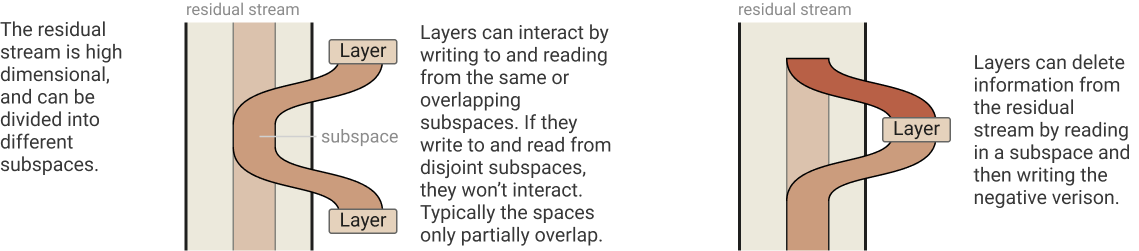
\includegraphics[width=0.75\linewidth]{assets/residual-stream.png}
    \caption{Schematic of the residual stream showing how attention heads contribute to different subspaces.}
    \label{fig:residual-stream}
\end{figure}

This has a concrete consequence for interpretability. Because heads write to subspaces, we can ask whether a given head's writing subspace overlaps with a subspace of interest, like the one defined by the label unembedding vectors. If $\operatorname{col}(W_O^{(k)})$ has no overlap with the label directions, the head cannot influence the model's choice between ``positive'' and ``negative.'' Conversely, a head whose writing subspace aligns well with the label directions is geometrically positioned to steer the prediction.

\subsection{The Unembedding and the Task Subspace}

The model's final prediction is produced by the \textit{unembedding matrix} $W_U \in \R^{d \times |\mathcal{V}|}$, which maps the residual stream vector at the final position into logits over the vocabulary. The logit for vocabulary token $v$ is simply the inner product $z_v = (W_U^{v})^\top x_{\text{final}}$, where $W_U^{v}$ is the column of $W_U$ corresponding to token $v$. This means that if a component writes a vector in a direction aligned with $W_U^{v}$, it directly increases the logit of token $v$.

For an ICL task with candidate label set $Y$ (e.g., $Y = \{\texttt{positive}, \texttt{negative}\}$ for SST-2), we extract the corresponding columns of $W_U$ and stack them into
\[
W_U^Y = \begin{bmatrix} W_U^{y_1} & W_U^{y_2} & \cdots & W_U^{y_{|Y|}} \end{bmatrix} \in \R^{d \times |Y|}.
\]
The column space $\mathrm{span}(W_U^Y)$ is the \emph{task subspace}: the low-dimensional part of the residual stream that directly controls the logits of the candidate labels. Any residual-stream component whose output has a large projection onto this subspace is writing information that specifically affects the model's choice among the task labels, rather than influencing unrelated vocabulary directions.

The orthogonal projection onto the task subspace is
\[
\operatorname{Proj}_{W_U^Y} = W_U^Y \bigl((W_U^Y)^\top W_U^Y\bigr)^{-1} (W_U^Y)^\top.
\]
This projector is the geometric tool behind both the TR and TL scores: it lets us decompose any head's output into a component that affects the task labels and a component that is irrelevant to them.

The \textbf{TR score} of a head measures the norm of this projected component, i.e.\ how much the head writes into the task subspace at all. The \textbf{TL score} then asks a finer question: within that projected component, does the head point in the contrastive direction $W_U^{y^*} - W_U^{y'}$ that favors the correct label $y^*$ over the incorrect ones $y' \in Y \setminus \{y^*\}$? Geometrically, TR captures alignment \emph{to} the task subspace, while TL captures rotation \emph{within} that subspace toward the correct answer. The precise formulations are given in Section~\ref{sec:methods}.

\subsection{Induction Heads}

Induction heads are attention heads that implement a simple but powerful pattern: they look back at previous occurrences of the current token (or context pattern) and copy what came next. In ICL, this manifests as a head attending from the query prediction position back to the label tokens in the demonstrations.

The mechanism was identified by \cite{TransformerCircuits} and studied extensively by \cite{InductionHeads}, who found it to be the primary driver of in-context learning in small models. The induction head (IH) score used in this project simply measures how much attention a head allocates from the final query position to all demo-label token positions, summed across demonstrations and prompts.

\subsection{TR vs.\ TL: Two Kinds of Heads}

The hypothesis from \cite{TSLA} is that some heads perform \textit{task recognition}, where they detect the structure of the demonstrations and steer the residual stream into the task subspace $\mathrm{span}(W_U^Y)$, without necessarily favoring the correct answer, while other heads perform \textit{task learning}, where they push the residual stream within that subspace toward the correct label direction. Concretely:

\begin{itemize}
    \item A \textbf{TR head} writes a large component into the task subspace (high $\|\operatorname{Proj}_{W_U^Y} a_{N,k}^{\,l}\|_2$): it steers the hidden state toward the label-semantic region, signaling that a particular classification task is being performed.
    \item A \textbf{TL head} writes a component that, within the task subspace, aligns with the correct-minus-incorrect direction (high TL score): it pushes the prediction toward the correct label specifically.
\end{itemize}

If these are actually different computations, we would expect different heads to score highly on TR vs.\ TL, with different layer distributions and different ablation effects. That is exactly what we test.

\begin{figure}[h!]
    \centering
    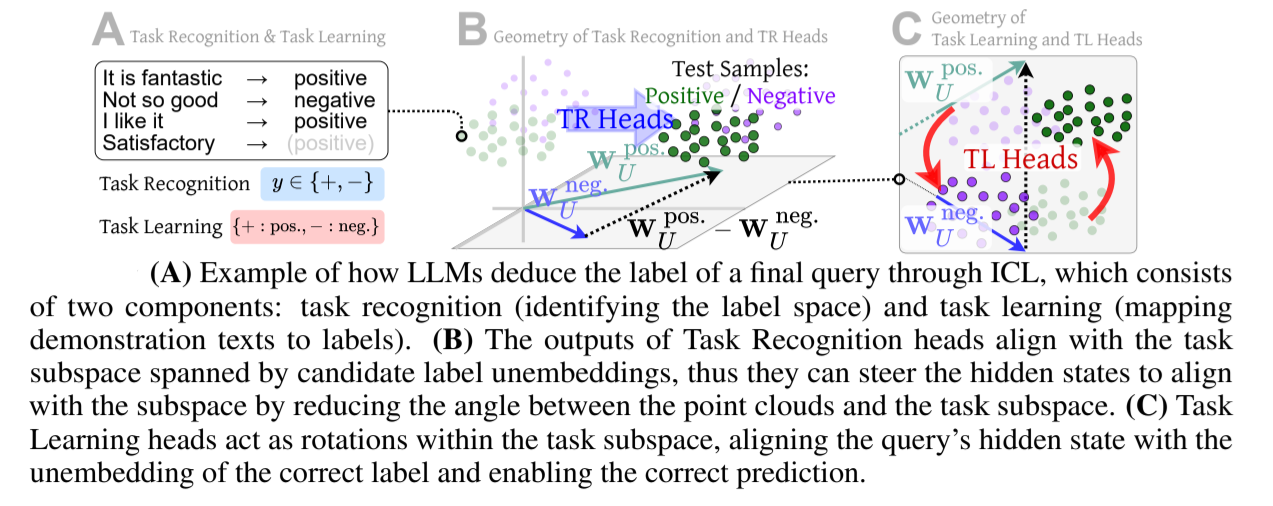
\includegraphics[width=0.75\linewidth]{assets/tl-tr-heads.png}
    \caption{Illustration of TR and TL head roles. TR heads project the residual stream into the task-label subspace, while TL heads steer within that subspace toward the correct label.}
    \label{fig:tl-tr-heads}
\end{figure}


% ============================================================================
% 5. PROBLEM STATEMENT AND REPRODUCTION GOAL
% ============================================================================
\section{Problem Statement and Reproduction Goal} \label{sec:problem}

The central question is: \textit{Can we identify and separate task recognition and task learning heads in an in-context learning setup, and does their behavior match the predictions from \cite{TSLA}?}

The original paper experiments on models with diverse architectures and sizes, including Llama3-8B, Llama3.1-8B, Llama3.2-3B, Qwen2-7B, Qwen2.5-32B, and Yi-34B, with results reported on Llama3-8B by default. It evaluates on seven datasets spanning sentiment (SST-2, MR), subjectivity (SUBJ), question classification (TREC), and natural language inference (SNLI, RTE, CB), all using 8-shot ICL. We use a single quantized model (\texttt{unsloth/Llama-3.2-3B-Instruct-bnb-4bit}) on a single dataset (SST-2) due to compute constraints. The goal is to test whether the core findings (TR/TL separation, TR-IH alignment, distinct layer distributions, and different ablation signatures) hold qualitatively under these scaled-down conditions.

Specifically, we aim to verify:
\begin{enumerate}
    \item TR heads overlap more with IH heads than TL heads do.
    \item TR and TL head sets are largely disjoint.
    \item Ablating TR, TL, and IH heads produces distinct patterns of degradation.
    \item TR heads concentrate in deeper layers than TL and IH heads.
    \item TR and TL heads attend to different parts of the prompt.
\end{enumerate}

% ============================================================================
% 6. METHODS AND APPROACHES
% ============================================================================
\section{Methods and Approaches} \label{sec:methods}

\subsection{Prompt Format}

We use a standard 8-shot ICL prompt for binary sentiment classification:

\begin{verbatim}
{sentence_1} Sentiment: {label_1}
{sentence_2} Sentiment: {label_2}
...
{sentence_8} Sentiment: {label_8}
{query_sentence} Sentiment:
\end{verbatim}

Eight balanced demonstrations (4 positive, 4 negative) are followed by a query sentence. The model's prediction is read from the logits at the final token position.

\subsection{Model}

We use \texttt{unsloth/Llama-3.2-3B-Instruct-bnb-4bit}, a 4-bit quantized (NF4) version of Meta's Llama-3.2-3B-Instruct. The model has 28 layers with 24 query attention heads per layer (grouped-query attention with 8 KV heads), giving $28 \times 24 = 672$ total heads, a hidden dimension of 3072, and a head dimension of 128. Full architectural specifications are given in Appendix~C.

Attention extraction requires \texttt{attn\_implementation="eager"} since SDPA does not support \texttt{output\_attentions}. Quantized weights in the output projection are dequantized on-the-fly for per-head output reconstruction.

\subsection{Head Scoring}

For each attention head $(l, k)$ at layer $l$ and head index $k$, we compute three scores across 50 scoring queries:

\paragraph{Task Subspace Logit Attribution (TSLA).}
Using the task subspace $\mathrm{span}(W_U^Y)$ and its orthogonal projection $\operatorname{Proj}_{W_U^Y}$ defined in Section~\ref{sec:background}, we score each attention head based on its output $a_{N,k}^{\,l} \in \mathbb{R}^{d}$ at the final query position $N$.

\paragraph{TR score.}
The paper defines the Task Recognition score of head \((l,k)\) as
\begin{equation}
\mathrm{TR}_{l,k}
=
\left\|
\operatorname{Proj}_{W_U^Y} a_{N,k}^{\,l}
\right\|_2.
\end{equation}
This score asks a simple geometric question: how much of the head's output lies inside the subspace spanned by the candidate-label unembeddings? A large TR score means that the head is primarily writing in directions that matter for representing the label set itself. In other words, such a head appears to be involved in \emph{recognizing the task}: it pushes the hidden state toward the semantic region associated with the demonstration labels, without yet specifying which label is correct for the current query. This matches the paper's interpretation that TR heads align hidden states with the task-label subspace.

\paragraph{TL score.}
Recognition of the label space is not enough for solving the task. The model must also choose the \emph{correct} label over the competing ones. Let \(y^* \in Y\) be the correct label for the query, and let \(Y \setminus \{y^*\}\) denote the incorrect candidates. The paper defines the Task Learning score as
\begin{equation}
\mathrm{TL}_{l,k}
=
\frac{
\operatorname{Ave}_{y' \in Y \setminus \{y^*\}}
\left(
(a_{N,k}^{\,l})^\top (W_U^{y^*} - W_U^{y'})
\right)
}{
\left\|
\operatorname{Proj}_{W_U^Y} a_{N,k}^{\,l}
\right\|_2 + \varepsilon
},
\end{equation}
where \(\varepsilon > 0\) is a small numerical constant for stability.

The numerator measures the \emph{logit gap} created by the head: it is large when the head increases the logit of the correct label relative to the incorrect ones. The denominator normalizes by the total amount of head output that already lies in the task subspace. This normalization is important. A head should not be considered a genuine TL head merely because it writes strongly in the label subspace; it should be considered a TL head only if, \emph{within that subspace}, it points in the contrastive direction that favors the correct label over the alternatives.

Geometrically, each difference vector \(W_U^{y^*} - W_U^{y'}\) lies inside \(\mathrm{span}(W_U^Y)\). Therefore, the TL score isolates the part of the projected head output that is aligned with the correct-versus-incorrect direction. This is why the paper interprets TL heads as performing a \emph{within-subspace rotation}: TR heads move the hidden state into the correct low-dimensional label-semantic subspace, while TL heads steer it inside that subspace toward the correct label and away from the competitors.

\paragraph{Binary SST-2 specialization.}
In our SST-2 setting, \(Y = \{\texttt{positive}, \texttt{negative}\}\). Hence the task subspace is two-dimensional (or lower, if the two unembedding vectors are not linearly independent), and the TL score simplifies to
\[
\mathrm{TL}_{l,k}
=
\frac{
(a_{N,k}^{\,l})^\top \bigl(W_U^{\texttt{pos}} - W_U^{\texttt{neg}}\bigr)
}{
\left\|
\operatorname{Proj}_{W_U^Y} a_{N,k}^{\,l}
\right\|_2 + \varepsilon
}
\]
when the correct label is \texttt{positive}, with the sign reversed when the correct label is \texttt{negative}. Thus, in the binary case, TR asks whether a head is writing about the sentiment-label space at all, while TL asks whether that head pushes specifically toward the correct sentiment.

\textbf{IH Score (Induction Head).} Let $s(Q_i)$ be the query prediction position for prompt $Q_i$, and let $I_i$ be the set of demo-label token positions:
\begin{equation}
\mathrm{IH}_{l,k} = \sum_{i} \sum_{j \in I_i} \mathrm{Attn}^{(l,k)}_{s(Q_i), j}
\end{equation}
This simply sums the attention weight from the prediction position to all demo-label tokens across all prompts.

\subsection{Head Selection}

We select the top 3\% of heads by each score. With 672 total heads, the top 3\% gives 20 heads per set: $\mathcal{H}_{\text{TR}}$, $\mathcal{H}_{\text{TL}}$, $\mathcal{H}_{\text{IH}}$. A matched-size random set $\mathcal{H}_{\text{Rand}}$ of 20 heads serves as a control.

\subsection{Ablation}

To test the causal role of each head set, we zero out the selected heads during inference. This is implemented via \texttt{register\_forward\_pre\_hook} on each head's output projection layer, which zeros the corresponding head's slice of the concatenated head output before the projection processes it. We then measure accuracy and TR ratio (fraction of predictions mapping to a valid task label) on a separate set of 200 evaluation queries.

% ============================================================================
% 7. DATA
% ============================================================================
\section{Data} \label{sec:data}

We use the SST-2 (Stanford Sentiment Treebank, binary) dataset from the GLUE benchmark, accessed via HuggingFace \texttt{datasets}. SST-2 is a binary sentiment classification dataset derived from Rotten Tomatoes movie reviews, with 67,349 training and 872 validation examples (full statistics in Appendix~C).

We split the data as follows:
\begin{itemize}
    \item \textbf{Demonstrations:} 8 examples sampled from the training split (4 positive, 4 negative), held fixed across all experiments. Seed = 42.
    \item \textbf{Scoring queries:} 50 examples from the validation split (offset 0), balanced by label. Used for computing TR, TL, and IH scores.
    \item \textbf{Evaluation queries:} 200 examples from the validation split (offset 50), non-overlapping with scoring queries. Used for ablation experiments.
\end{itemize}

Labels are mapped as: SST-2 label 0 $\to$ ``negative,'' label 1 $\to$ ``positive.'' The two label words serve as both prompt labels and the basis for the task subspace in the unembedding space.

% ============================================================================
% 8. EXPERIMENTAL SETUP
% ============================================================================
\section{Experimental Setup} \label{sec:setup}

\begin{itemize}
    \item \textbf{Hardware:} Kaggle GPU runtime with NVIDIA P100 (16 GB VRAM).
    \item \textbf{Software:} PyTorch, HuggingFace Transformers, bitsandbytes $\geq$ 0.46.1 for 4-bit quantization.
    \item \textbf{Model:} \texttt{unsloth/Llama-3.2-3B-Instruct-bnb-4bit} (28 layers, 24 heads/layer, 672 total heads, hidden dim 3072, head dim 128).
    \item \textbf{Scoring queries:} 50 prompts for head identification. Scores averaged (TR, TL) or summed (IH) across prompts.
    \item \textbf{Evaluation queries:} 200 prompts for ablation.
    \item \textbf{Top-$k$ threshold:} 3\% = 20 heads.
    \item \textbf{Attention mode:} \texttt{eager} (required for attention weight extraction with \texttt{output\_attentions=True}).
    \item \textbf{Caching:} All intermediate results cached to disk to avoid recomputation.
    \item \textbf{Seed:} 42 for all random operations.
    \item \textbf{Code:} All source code, configuration files, and the experiment notebook are available at \url{https://github.com/TejasNC/task-subspace-logit-attribution}.
\end{itemize}

Note that this is a \emph{scaled qualitative reproduction}, not a full exact replication. Due to compute constraints, we use a single quantized model on a single dataset with fewer scoring queries than the original paper. The goal is to test whether the paper's core qualitative findings hold under these reduced conditions, not to match the original numbers exactly.

% ============================================================================
% 9. EXPERIMENTS
% ============================================================================
\section{Experiments} \label{sec:experiments}

\subsection{Experiment 1: TR, TL, and IH Head Identification}

\textbf{Question:} Which heads score highest on TR, TL, and IH metrics, and do their top sets overlap as predicted?

\textbf{Method:} For each of 50 scoring queries, we build an 8-shot ICL prompt, run a forward pass with attention extraction and value-state hooks, compute per-head TR, TL, and IH scores, and aggregate across queries. The top 20 heads by each score form $\mathcal{H}_{\text{TR}}$, $\mathcal{H}_{\text{TL}}$, and $\mathcal{H}_{\text{IH}}$.

\textbf{Expectation:} TR heads should overlap more with IH heads than TL heads do, because task recognition involves attending to demonstration labels (an induction-like pattern). TR and TL sets should be largely disjoint.

\subsection{Experiment 2: Overlap and Specialization}

\textbf{Question:} How related are the TR, TL, and IH head rankings, not just at the top 3\%, but across all 672 heads?

\textbf{Method:} We compute Jaccard overlap between top head sets, Kendall $\tau$ and Spearman $\rho$ rank correlations over all heads, and conditional mean percentile analysis (for the top $p$\% IH heads, what is their average percentile under TR and TL rankings?).

\textbf{Expectation:} TR-IH similarity should be stronger than TL-IH across all metrics.

\subsection{Experiment 3: Ablation Study}

\textbf{Question:} What happens to model performance when we zero out different head sets?

\textbf{Method:} We zero out each head set ($\mathcal{H}_{\text{TR}}$, $\mathcal{H}_{\text{TL}}$, $\mathcal{H}_{\text{IH}}$, $\mathcal{H}_{\text{Rand}}$) during inference on 200 evaluation queries. We measure accuracy and TR ratio.

\textbf{Expectation:} TR ablation should reduce both accuracy and TR ratio. TL ablation should reduce accuracy more than TR ratio (the model still ``knows'' it is doing sentiment, but picks the wrong label). Random ablation should have minimal impact.

\subsection{Experiment 4: Layer-wise Distribution}

\textbf{Question:} Where in the network do TR, TL, and IH heads concentrate?

\textbf{Method:} For each head set, compute the mean, median, and standard deviation of layer indices. Use Mann-Whitney U tests to compare distributions.

\textbf{Expectation:} TR heads should occur in deeper layers than TL and IH heads. TL and IH heads should have more similar layer distributions.

\subsection{Experiment 5: Attention Distribution}

\textbf{Question:} What parts of the prompt do different head types attend to from the prediction position?

\textbf{Method:} For each head in each set, measure the total attention from the final query position to: (a) demo-label tokens, (b) query-sentence tokens, (c) all other tokens. Average across prompts and heads within each type.

\textbf{Expectation:} TR heads should allocate more attention to demo-label tokens. TL heads should attend more to query-sentence tokens. Random heads should show no structured pattern.

% ============================================================================
% 10. RESULTS AND DISCUSSION
% ============================================================================
\section{Results and Discussion} \label{sec:results}

\subsection{Experiment 1: Head Identification}

The top 20 TR, TL, and IH heads were identified by ranking all 672 heads using their aggregated scores over the scoring prompts. At the most basic level, the overlap pattern already matches the central qualitative claim of the paper: the TR-IH overlap was \textbf{4/20}, whereas the TL-IH overlap was only \textbf{1/20}. Thus, induction-like behavior is much more strongly associated with \emph{task recognition} than with \emph{task learning}.

This observation is important conceptually. In the paper, and as is usually the case in mechanistic interpretability literature, induction heads are not interpreted as heads that directly solve the classification problem by amplifying the correct label. Rather, they are argued to contribute mainly by helping the model \emph{recognize the task structure} encoded by the demonstrations, especially the label space itself. Our result is consistent with that picture: IHs appear to overlap primarily with the heads that align hidden states with the task-label subspace, not with the heads that perform the finer discrimination toward the correct answer.

Notably,
\[
\mathcal{H}_{\mathrm{TR}} \cap \mathcal{H}_{\mathrm{TL}} = \emptyset,
\]
that is, there is zero overlap between the top TR and top TL sets at the chosen threshold. This is a particularly strong form of evidence for specialization. If the same heads were jointly responsible for both task recognition and task learning, one would expect at least some overlap among the highest-ranked heads. Instead, the complete separation suggests that these two functions are implemented by distinct components, even though both ultimately contribute to the final in-context prediction.

Taken together, these results support the paper's broader mechanistic story. In-context learning does not appear to be carried out by a single homogeneous class of ``important heads.'' Rather, it decomposes into at least two separable roles: first, identifying the relevant task-label geometry from the demonstrations, and second, using the query semantics to move toward the correct label within that geometry. The fact that IHs align with TR much more than with TL further sharpens this picture: induction-style copying seems to be more about \emph{establishing the right label space} than about \emph{making the final decision}.

A final caveat is that overlap at the top \(3\%\) is a deliberately strict criterion. At such a narrow threshold, even a difference of a few shared heads can be meaningful. Therefore, these top-set overlaps should not be read in isolation, but as the first indication of a deeper pattern that is better validated by the subsequent rank-correlation, ablation, and layer-wise analyses.

\begin{figure}[h!]
    \centering
    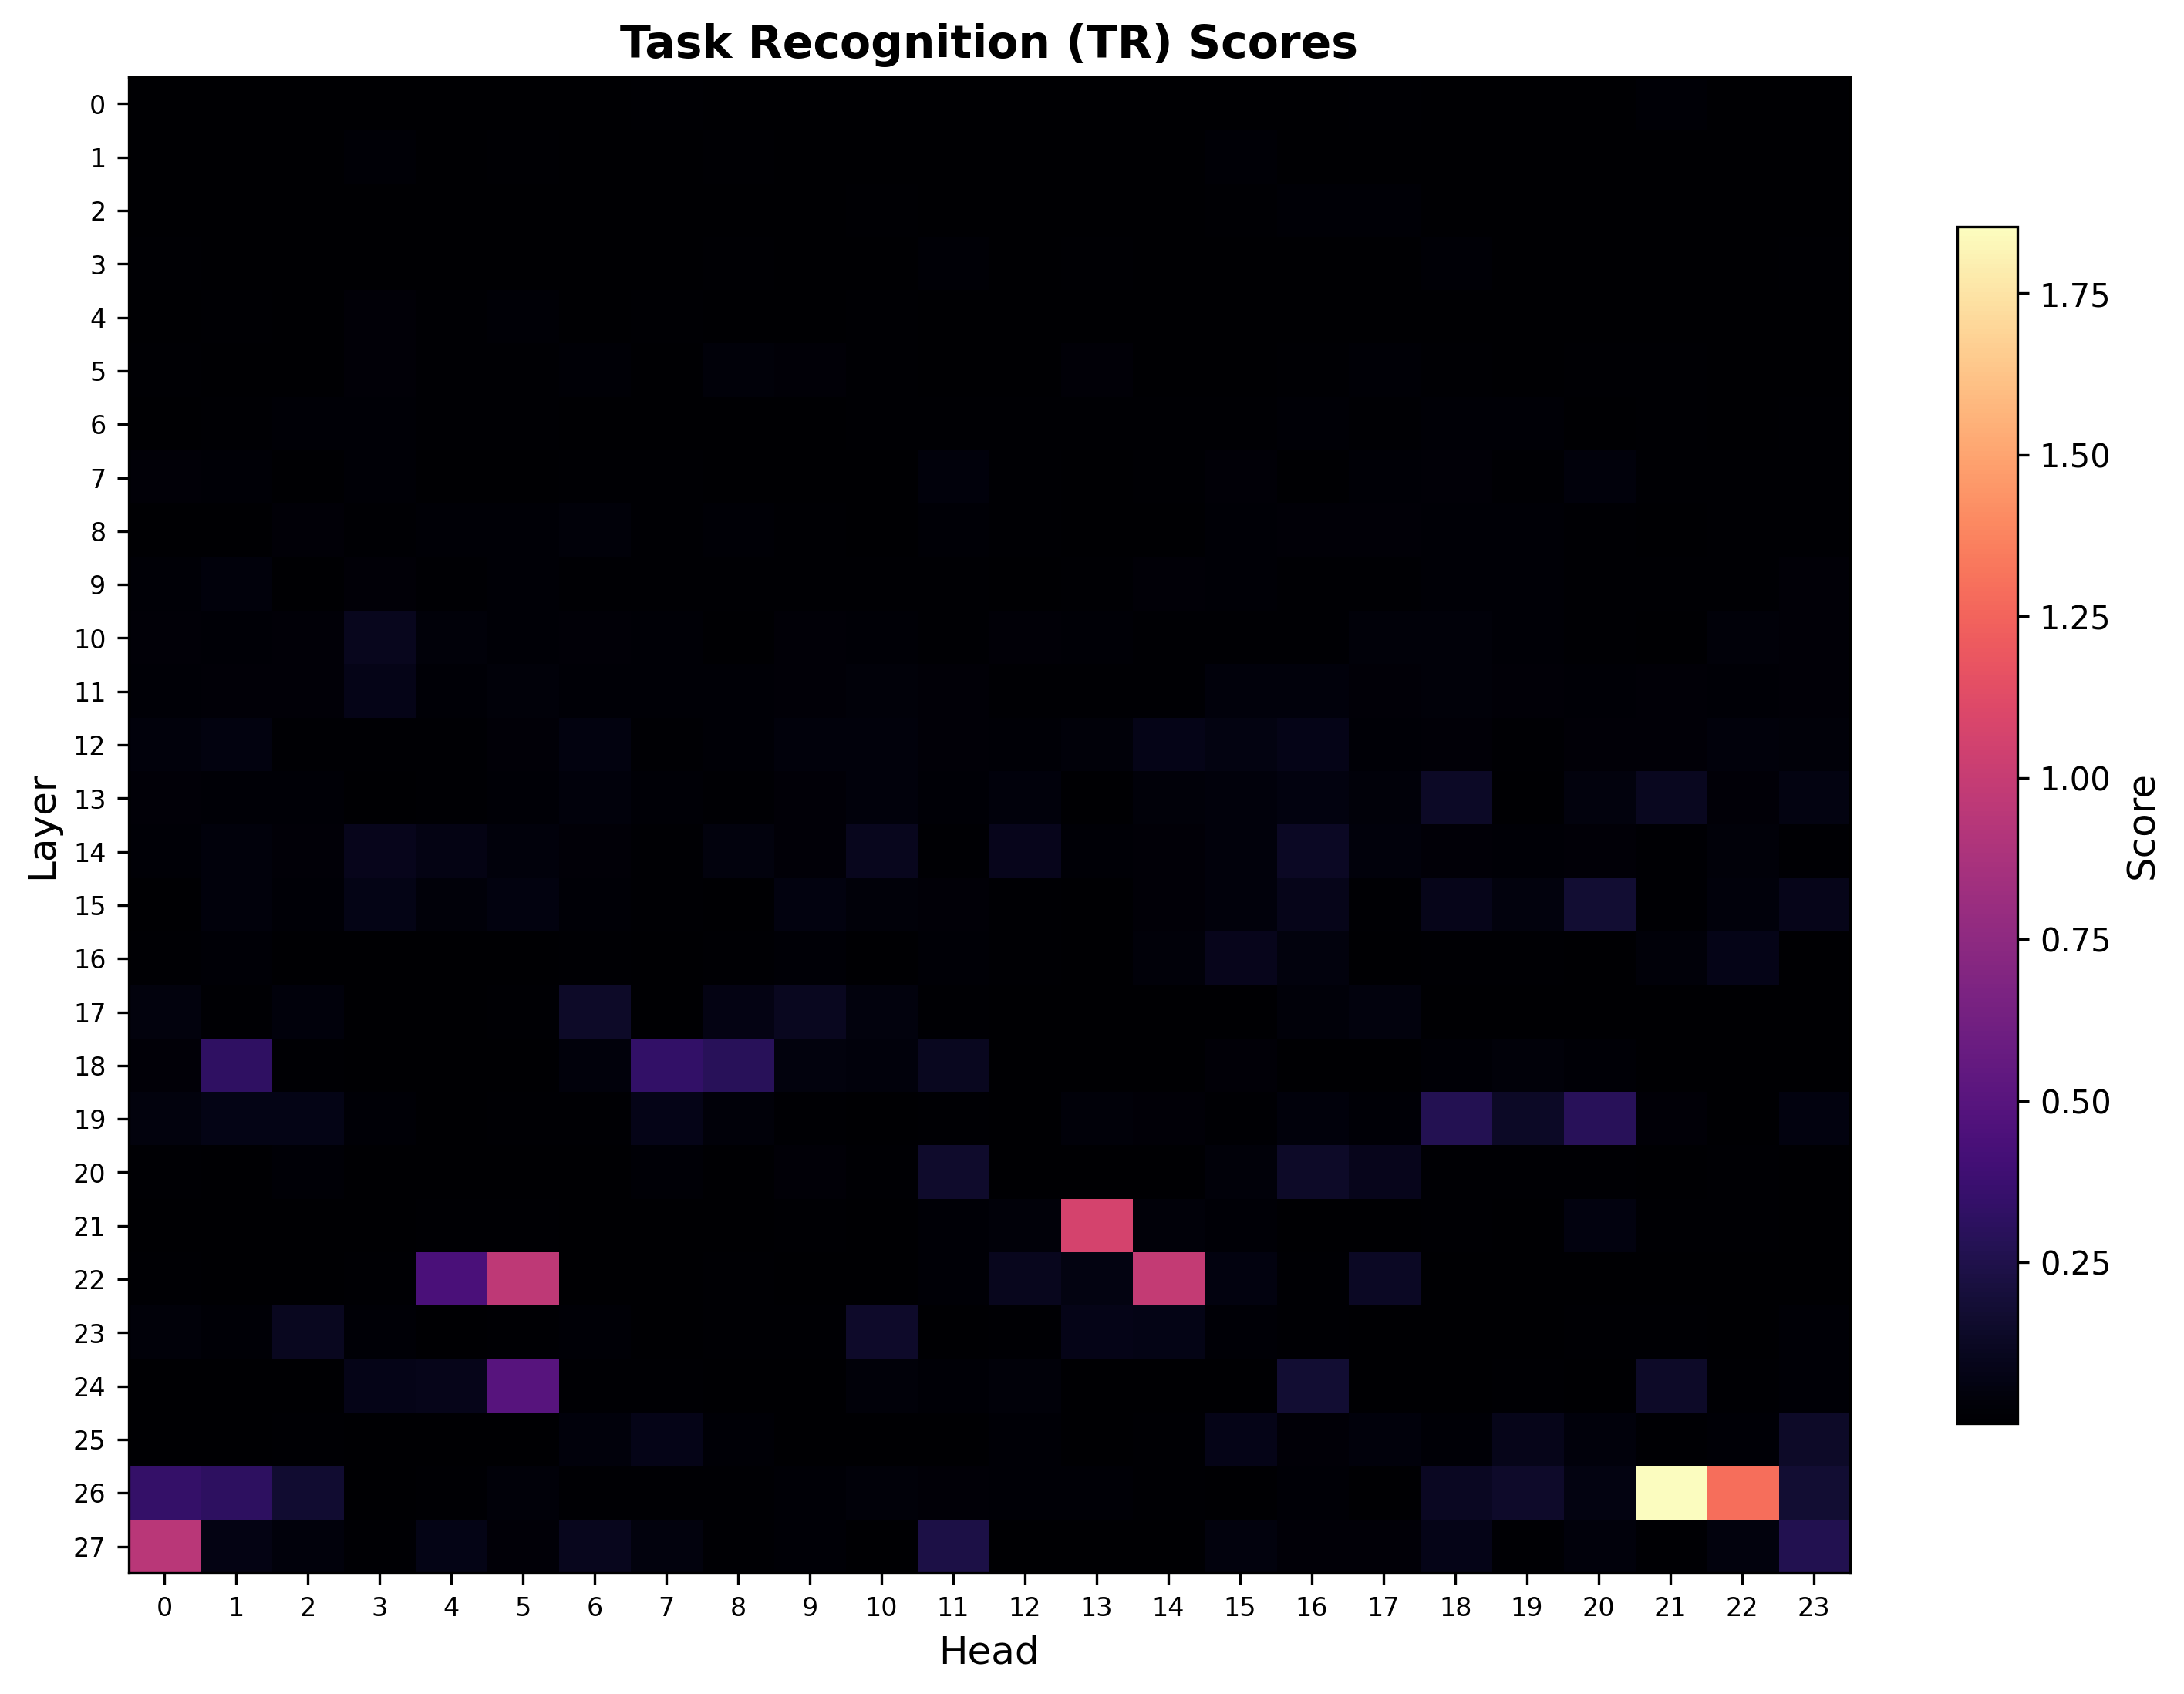
\includegraphics[width=0.32\linewidth]{assets/experiment-1-tr-heatmap.png}\hfill
    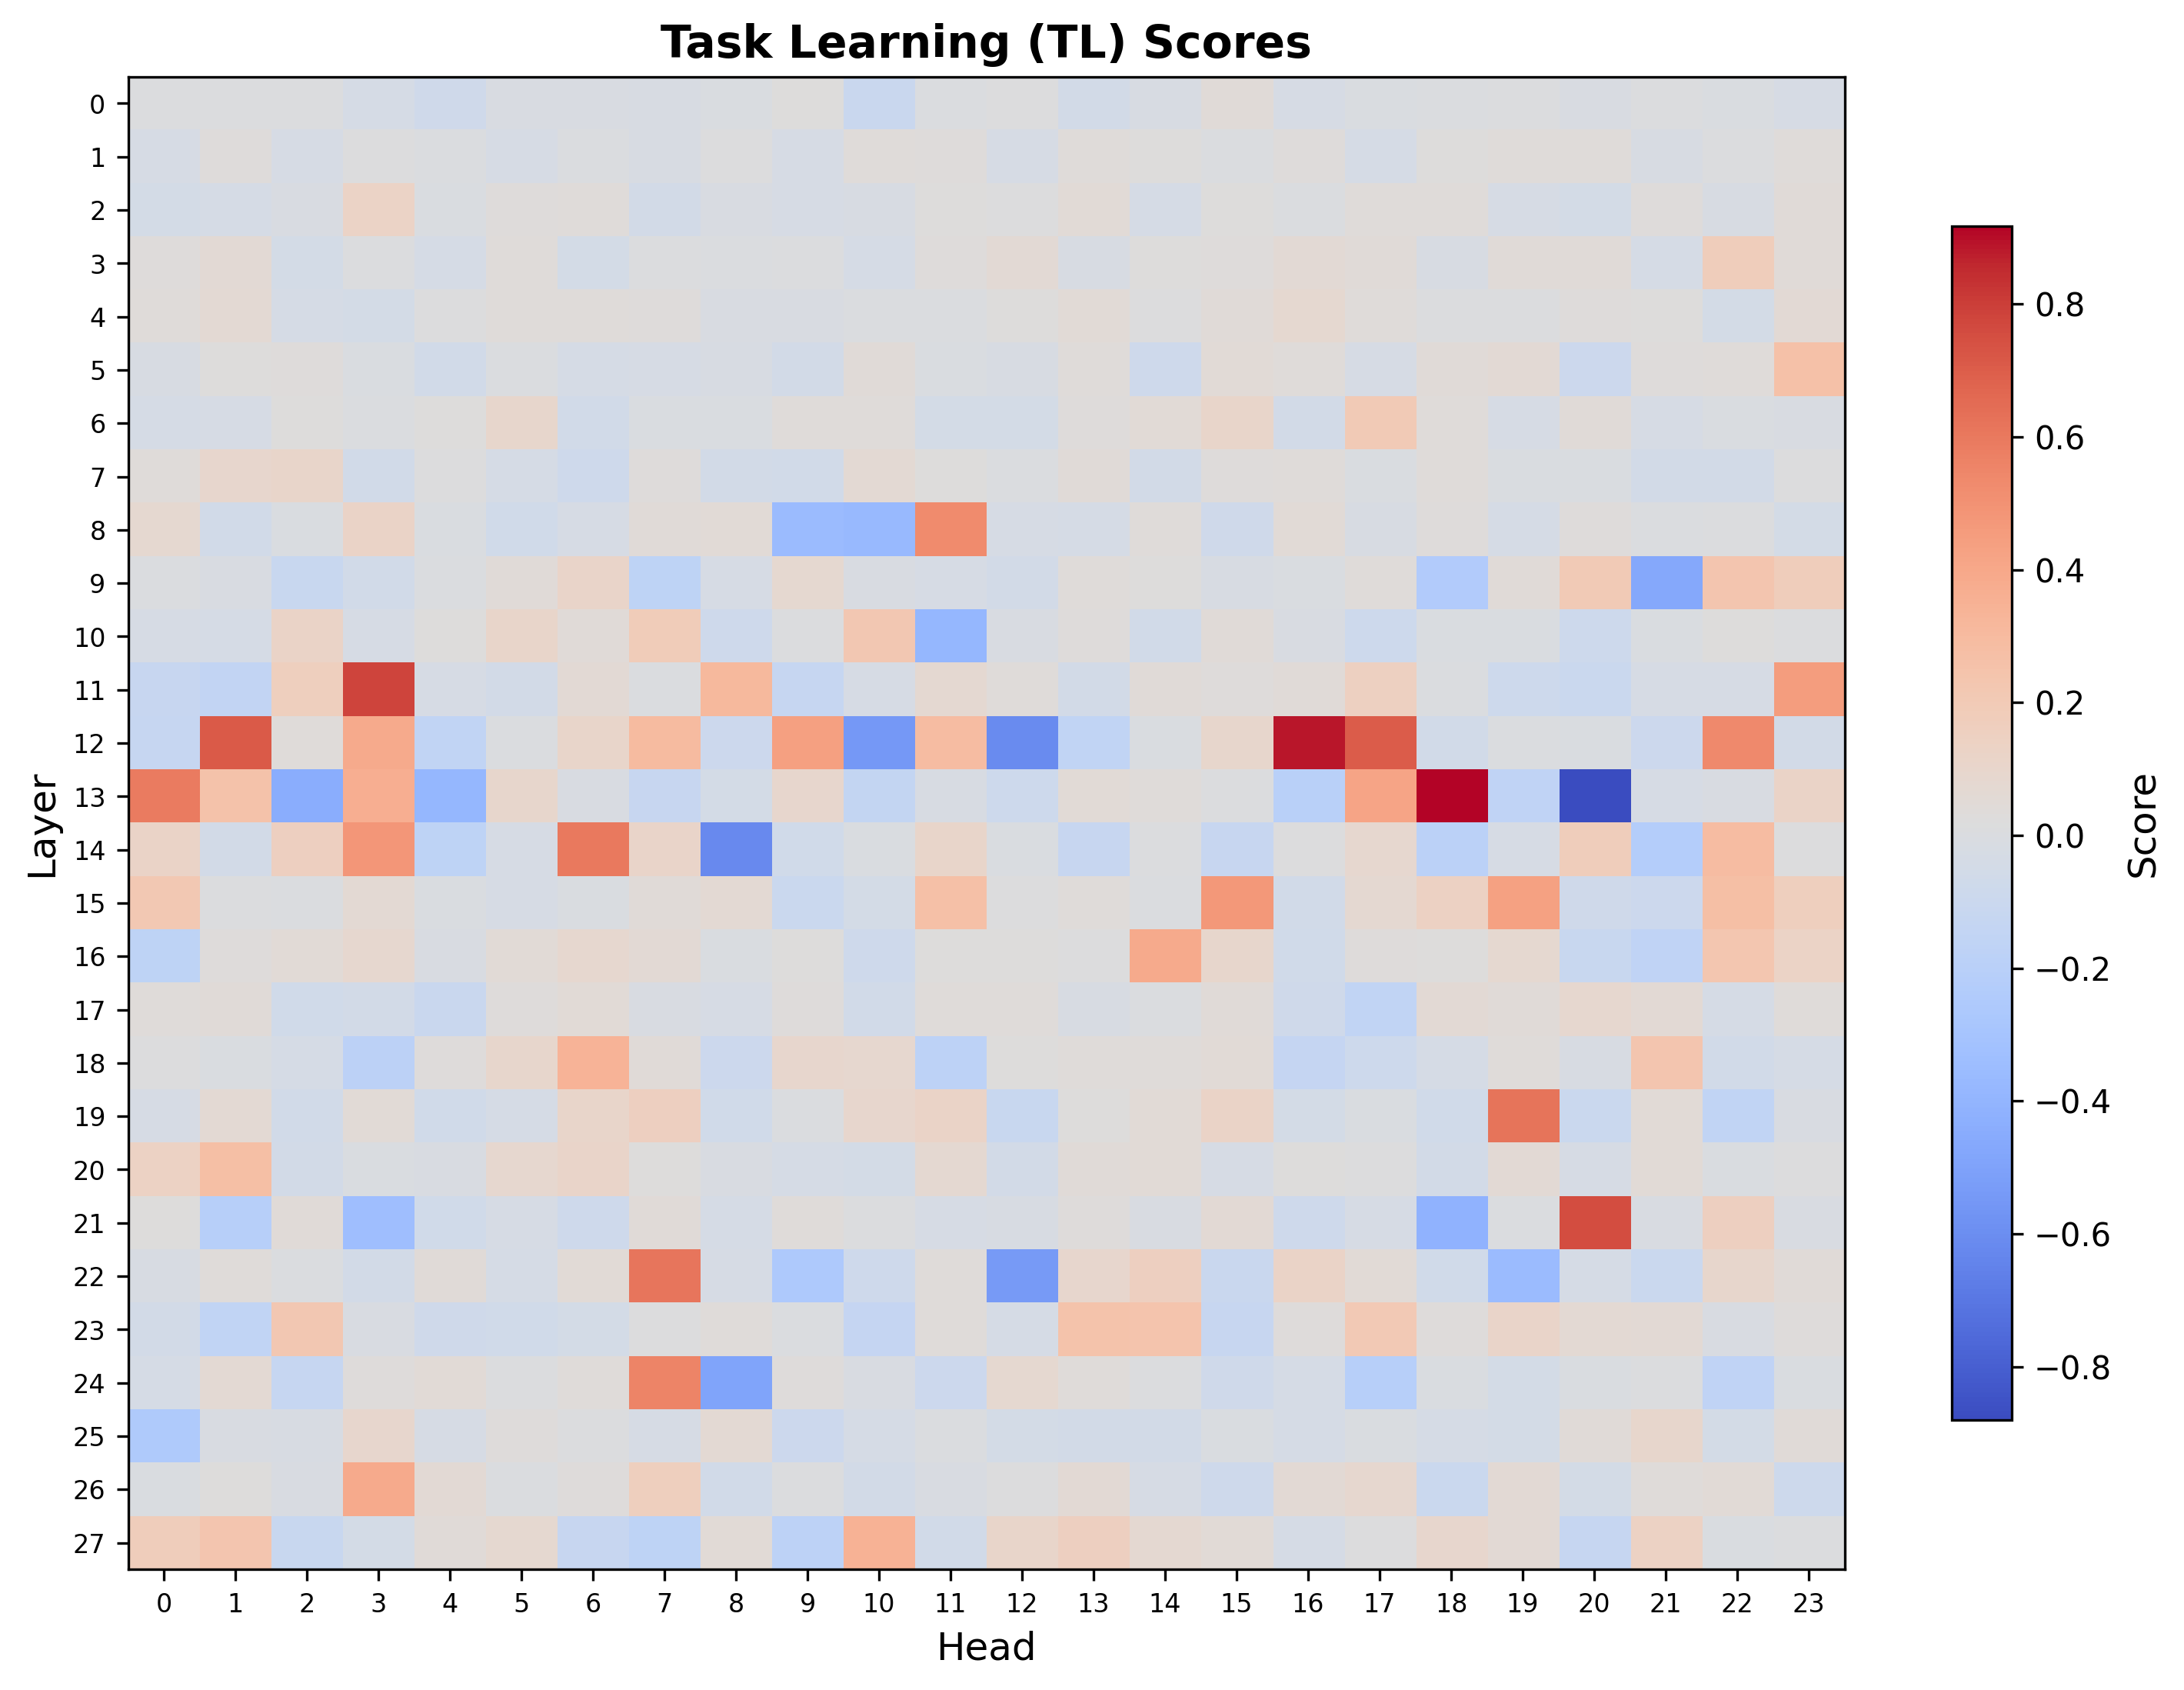
\includegraphics[width=0.32\linewidth]{assets/experiment-1-tl-heatmap.png}\hfill
    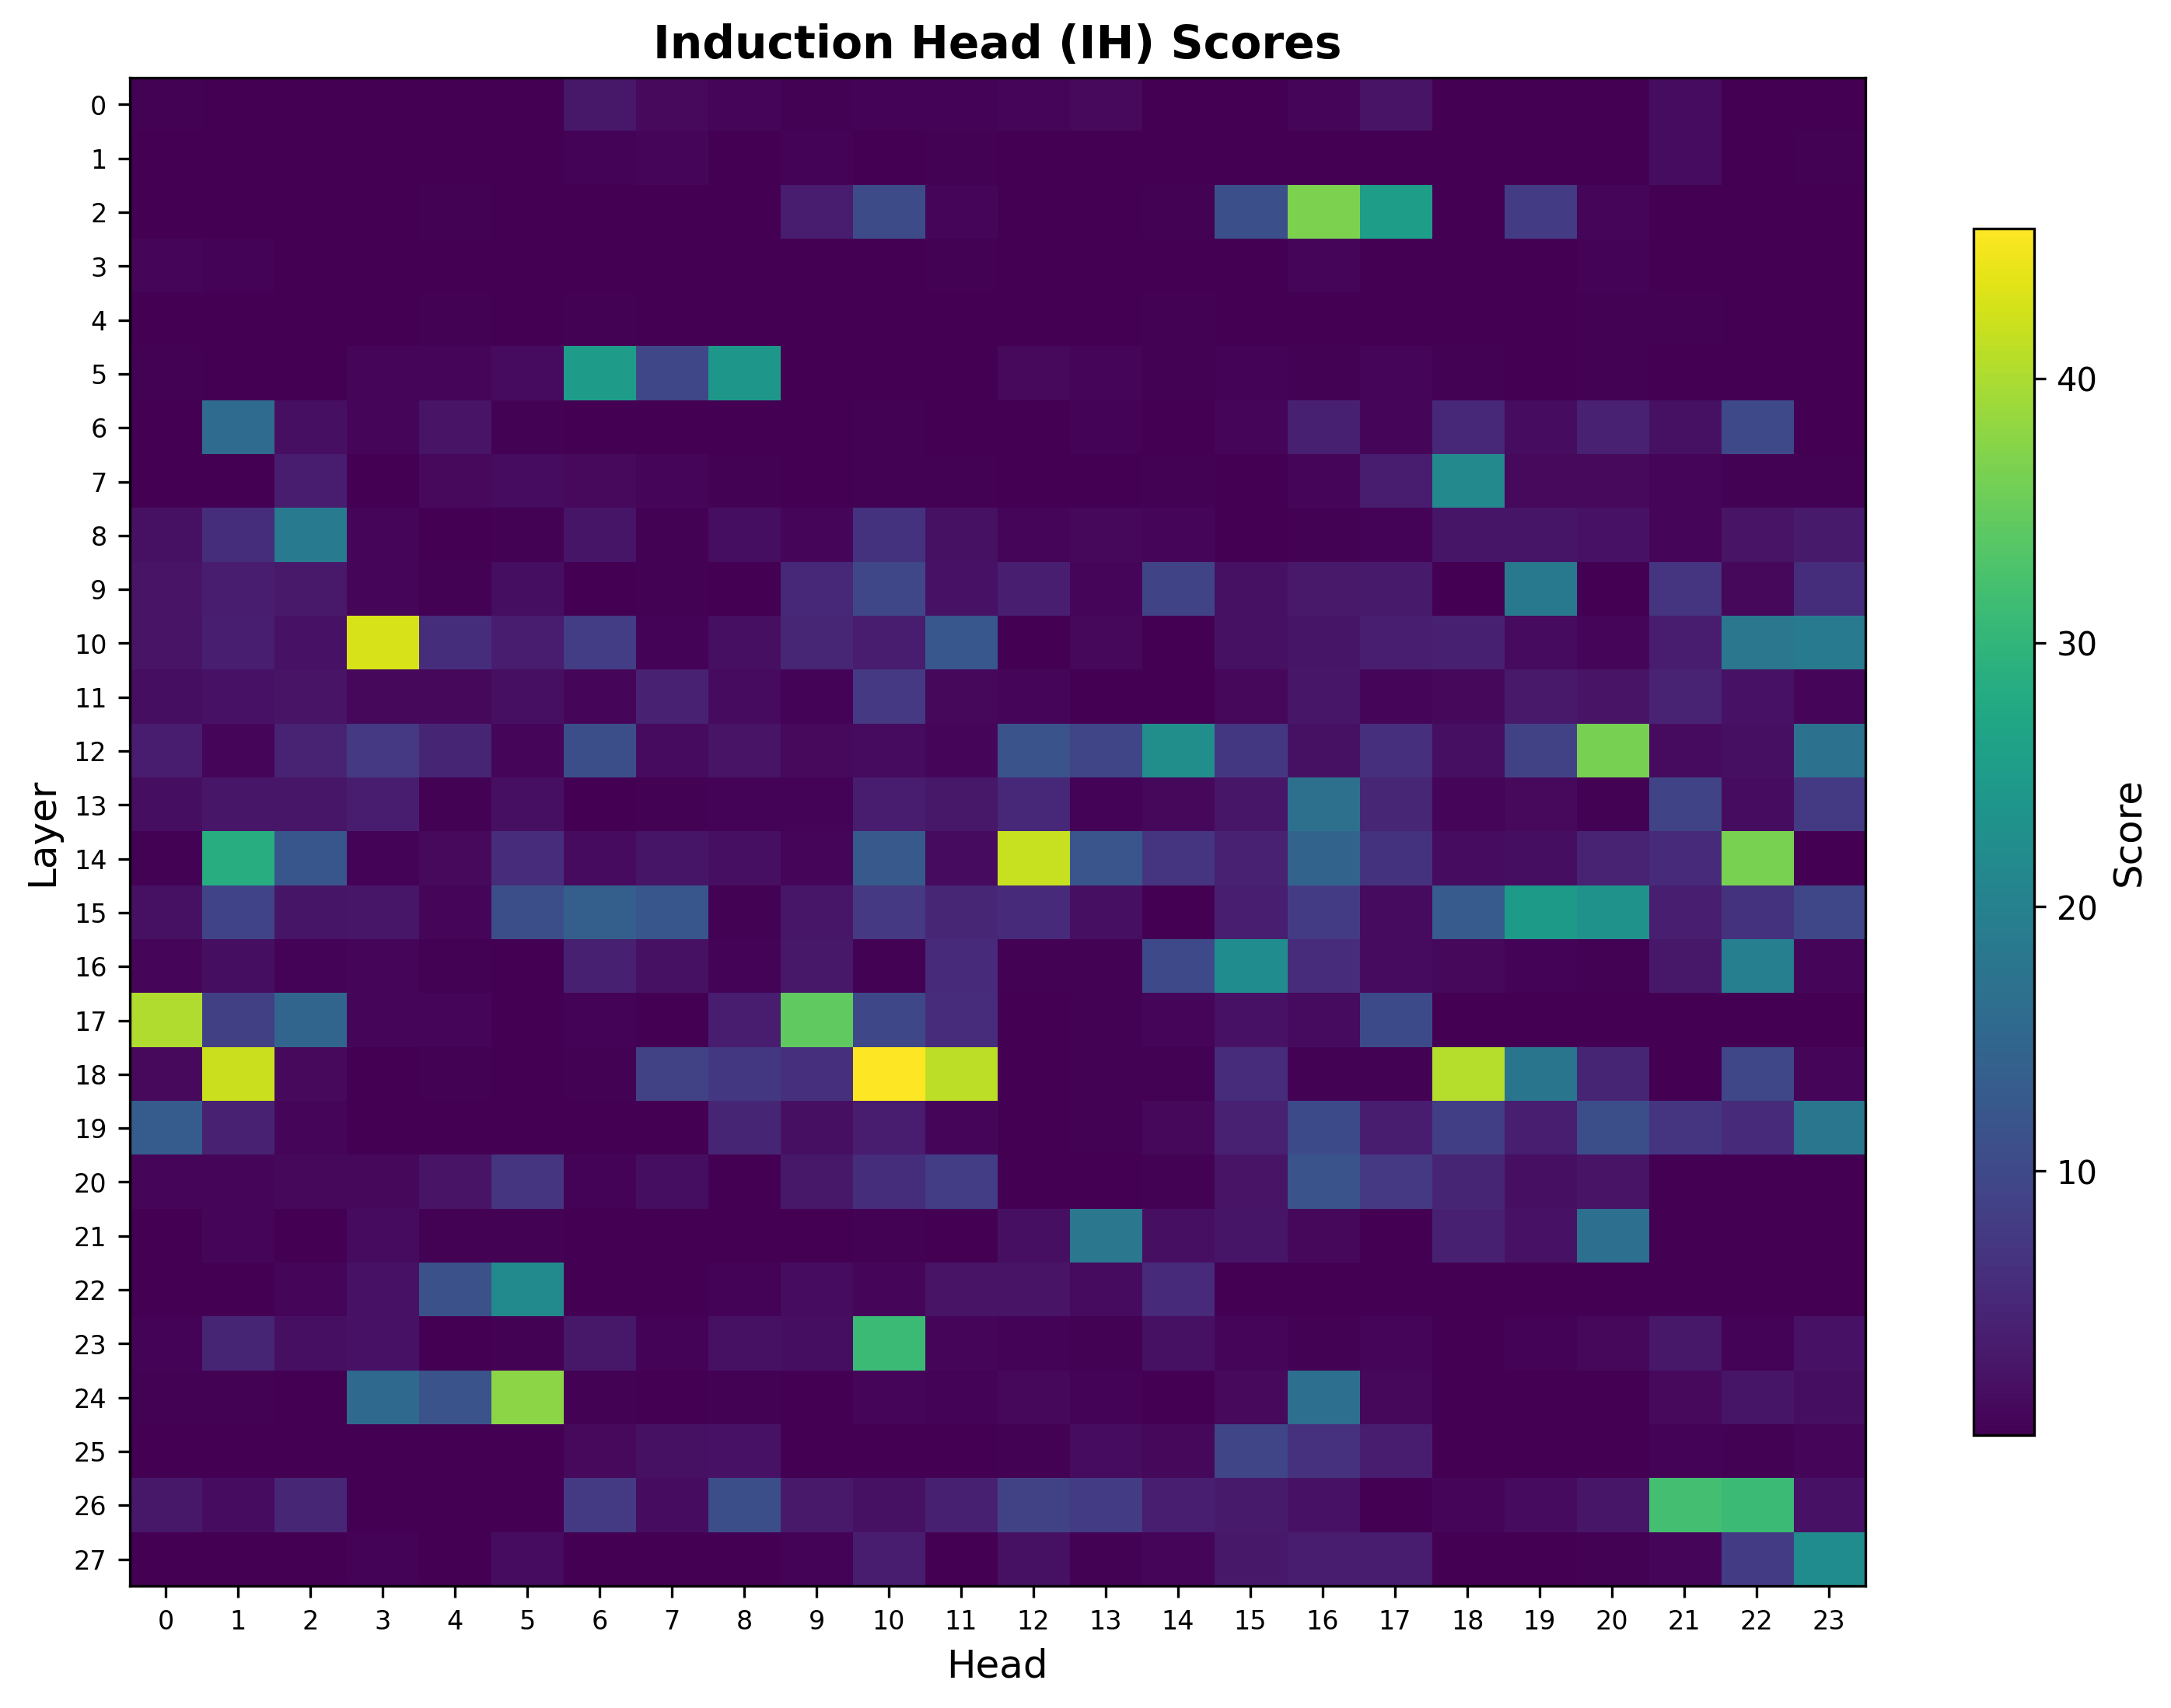
\includegraphics[width=0.32\linewidth]{assets/experiment-1-ih-heatmap.png}
    \caption{Experiment 1 per-head score heatmaps (layer $\times$ head index) for TR (left), TL (center), and IH (right). Brighter cells indicate higher scores. TR activity concentrates in deep layers, while TL and IH heads are spread across middle layers.}
    \label{fig:exp1-heatmaps}
\end{figure}

\subsection{Experiment 2: Overlap and Specialization}

% Table: overlap metrics here
\begin{table}[h]
\centering
\caption{Overlap and rank correlation metrics between head-score rankings.}
\begin{tabular}{lccc}
\toprule
\textbf{Metric} & \textbf{TR vs TL} & \textbf{TR vs IH} & \textbf{TL vs IH} \\
\midrule
Jaccard (top 3\%) & 0.0000 & 0.1111 & 0.0256 \\
Kendall $\tau$ & 0.0089 & 0.3836 & $-$0.0174 \\
Spearman $\rho$ & 0.0152 & 0.5451 & $-$0.0291 \\
\bottomrule
\end{tabular}
\label{tab:overlap}
\end{table}

The results in Table~\ref{tab:overlap} sharpen the conclusion of Experiment~1 by showing that the relationship between TR heads and IHs is not merely an artifact of the top-20 sets, but persists across the \emph{entire} ranking of all 672 heads. The strongest signal is the TR--IH correlation: both Kendall's \(\tau = 0.3836\) and Spearman's \(\rho = 0.5451\) indicate a substantial positive association between the two rankings. In contrast, the corresponding TR--TL and TL--IH correlations are essentially zero. Thus, heads that score highly as induction-like also tend to score highly as task-recognition heads, whereas task-learning heads are globally ranked in a largely unrelated way.

This distinction is mechanistically meaningful. In the paper, IHs are argued to support ICL mainly by helping the model identify the relevant label space from the demonstrations, rather than by directly performing the final correct-versus-incorrect discrimination. Our results fit this interpretation closely. The fact that the TR ranking is globally aligned with the IH ranking, while the TL ranking is not, suggests that induction-style behavior is much more tightly coupled to \emph{recognizing} the task structure than to \emph{solving} the task inside that structure.

The Jaccard coefficients provide a complementary, top-level view. Even under the strict top-\(3\%\) threshold, TR--IH overlap remains clearly larger than TL--IH overlap, while TR--TL overlap is exactly zero. Since these top sets are very small, even a modest Jaccard value is informative; what matters here is the \emph{relative} pattern:
\[
J(\mathrm{TR},\mathrm{IH}) \gg J(\mathrm{TL},\mathrm{IH}), \qquad
J(\mathrm{TR},\mathrm{TL}) = 0.
\]
This again supports the specialization picture proposed in the paper: TR heads share substantial common structure with IHs, while TL heads form a distinct class.

Another useful way to read these results is that they bridge local and global notions of specialization. The Jaccard index only asks whether the very top heads overlap, while Kendall's \(\tau\) and Spearman's \(\rho\) ask whether the \emph{overall ordering} of heads agrees. Here both views tell the same story. The agreement is therefore not a fragile threshold effect; it reflects a broader alignment between the TR and IH mechanisms throughout the network.

Overall, the overlap and correlation analysis provides stronger evidence than raw top-set overlap alone. It shows that the paper's central claim is not just that ``some IHs are also TR heads,'' but that the entire \emph{induction-head-like axis} in the model is much closer to task recognition than to task learning. This makes the later causal experiments easier to interpret: if ablating IH-related heads harms task recognition disproportionately, that effect is not surprising, because the ranking structure already indicates that IHs live much closer to the TR channel than to the TL channel.

\begin{figure}[h!]
    \centering
    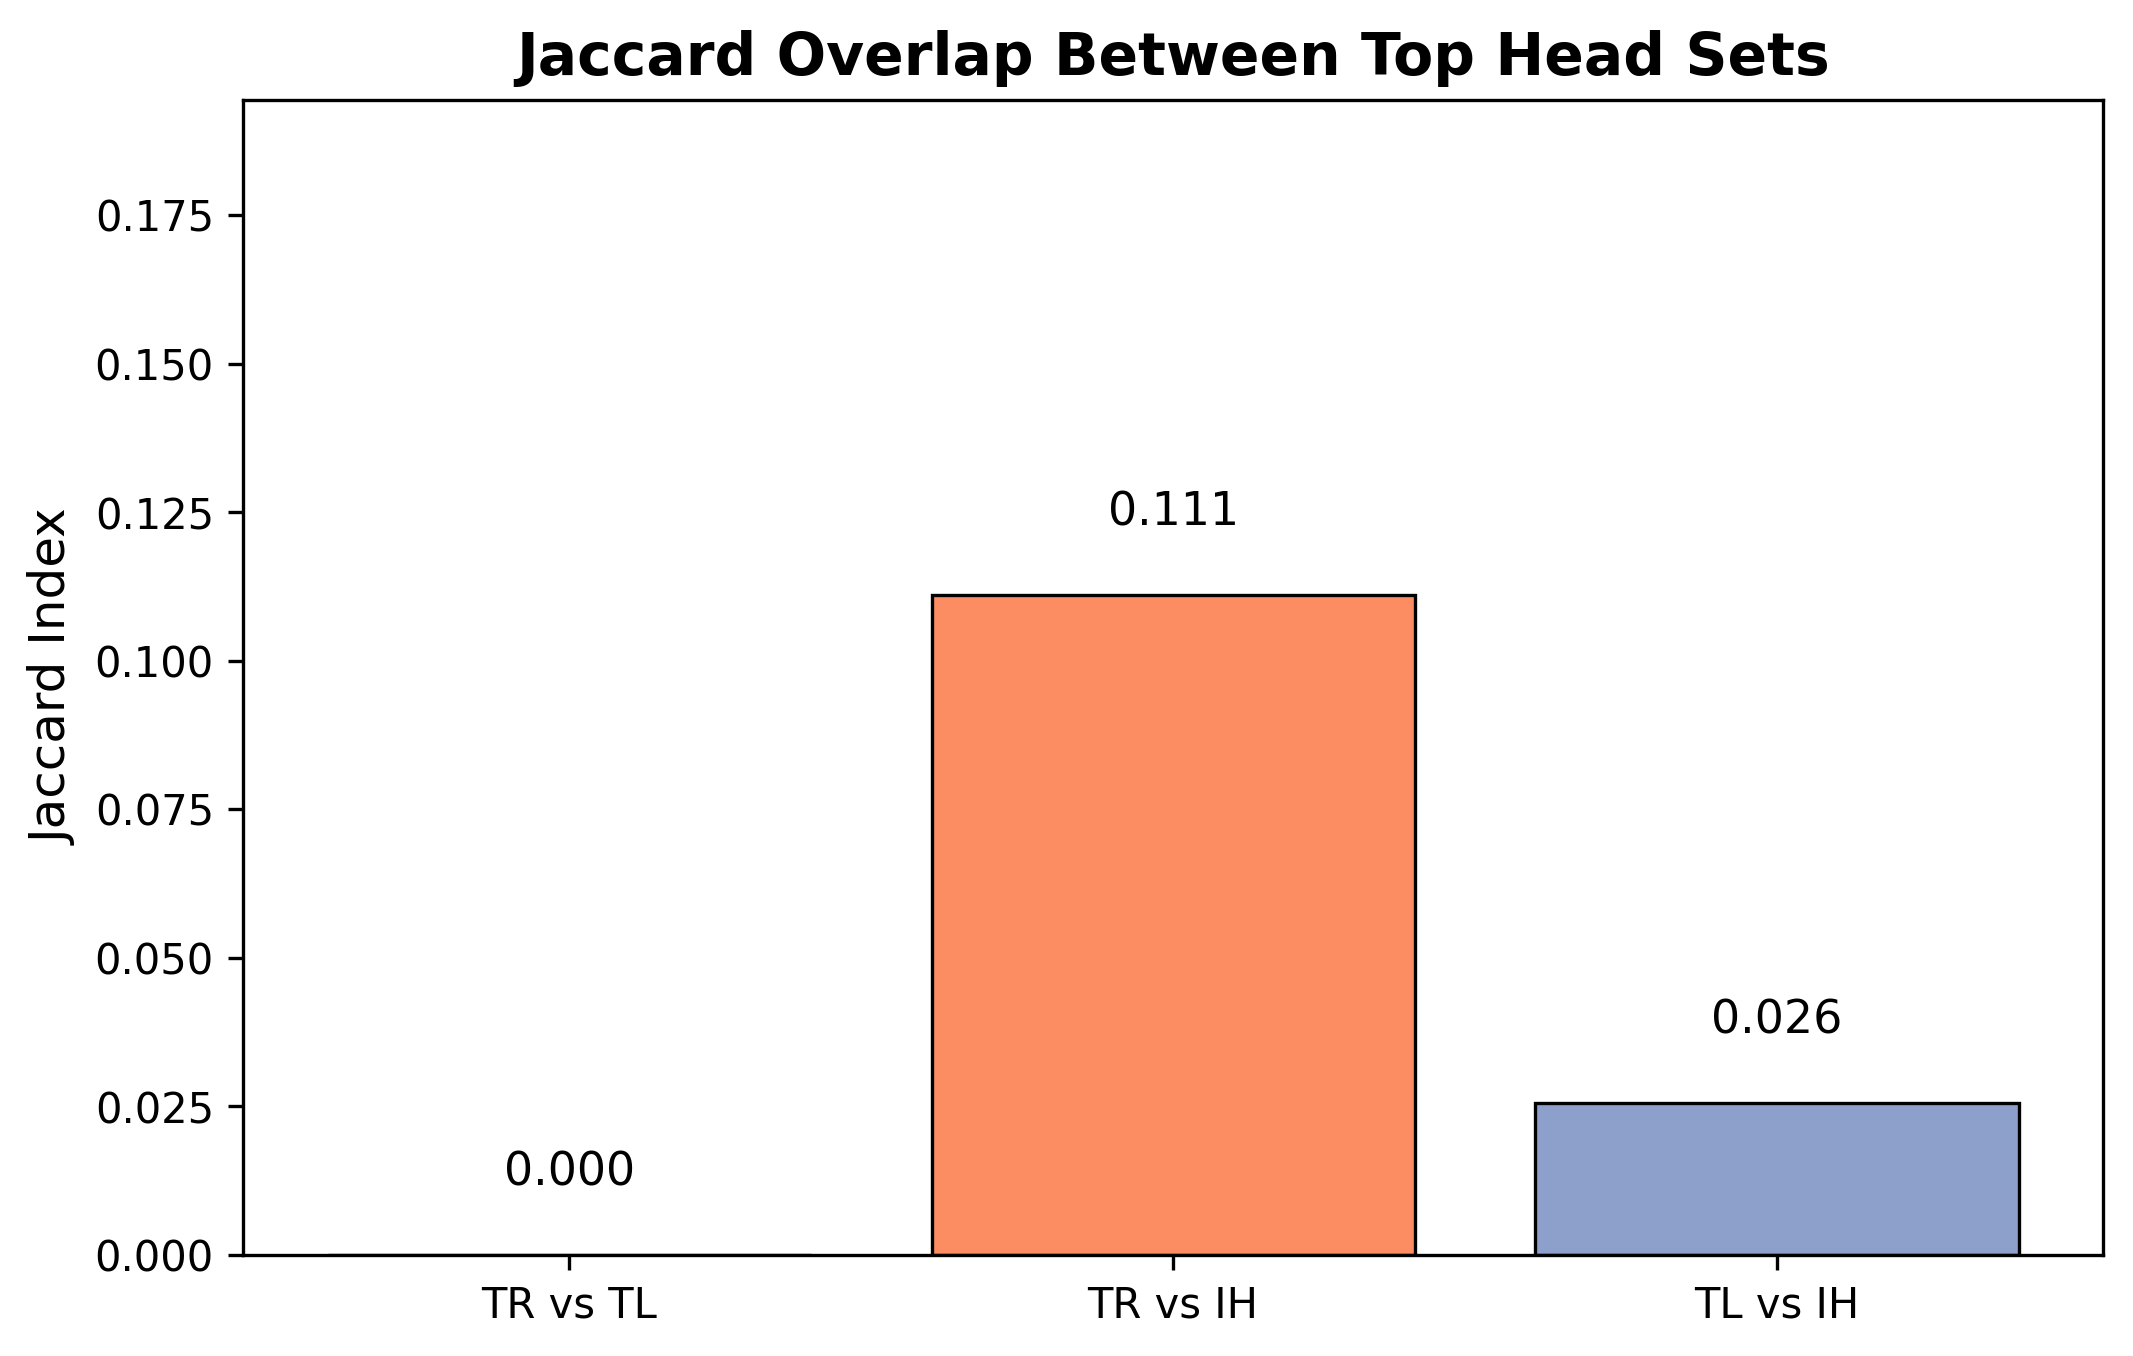
\includegraphics[width=0.32\linewidth]{assets/experiment-2-jacard-similarity.png}\hfill
    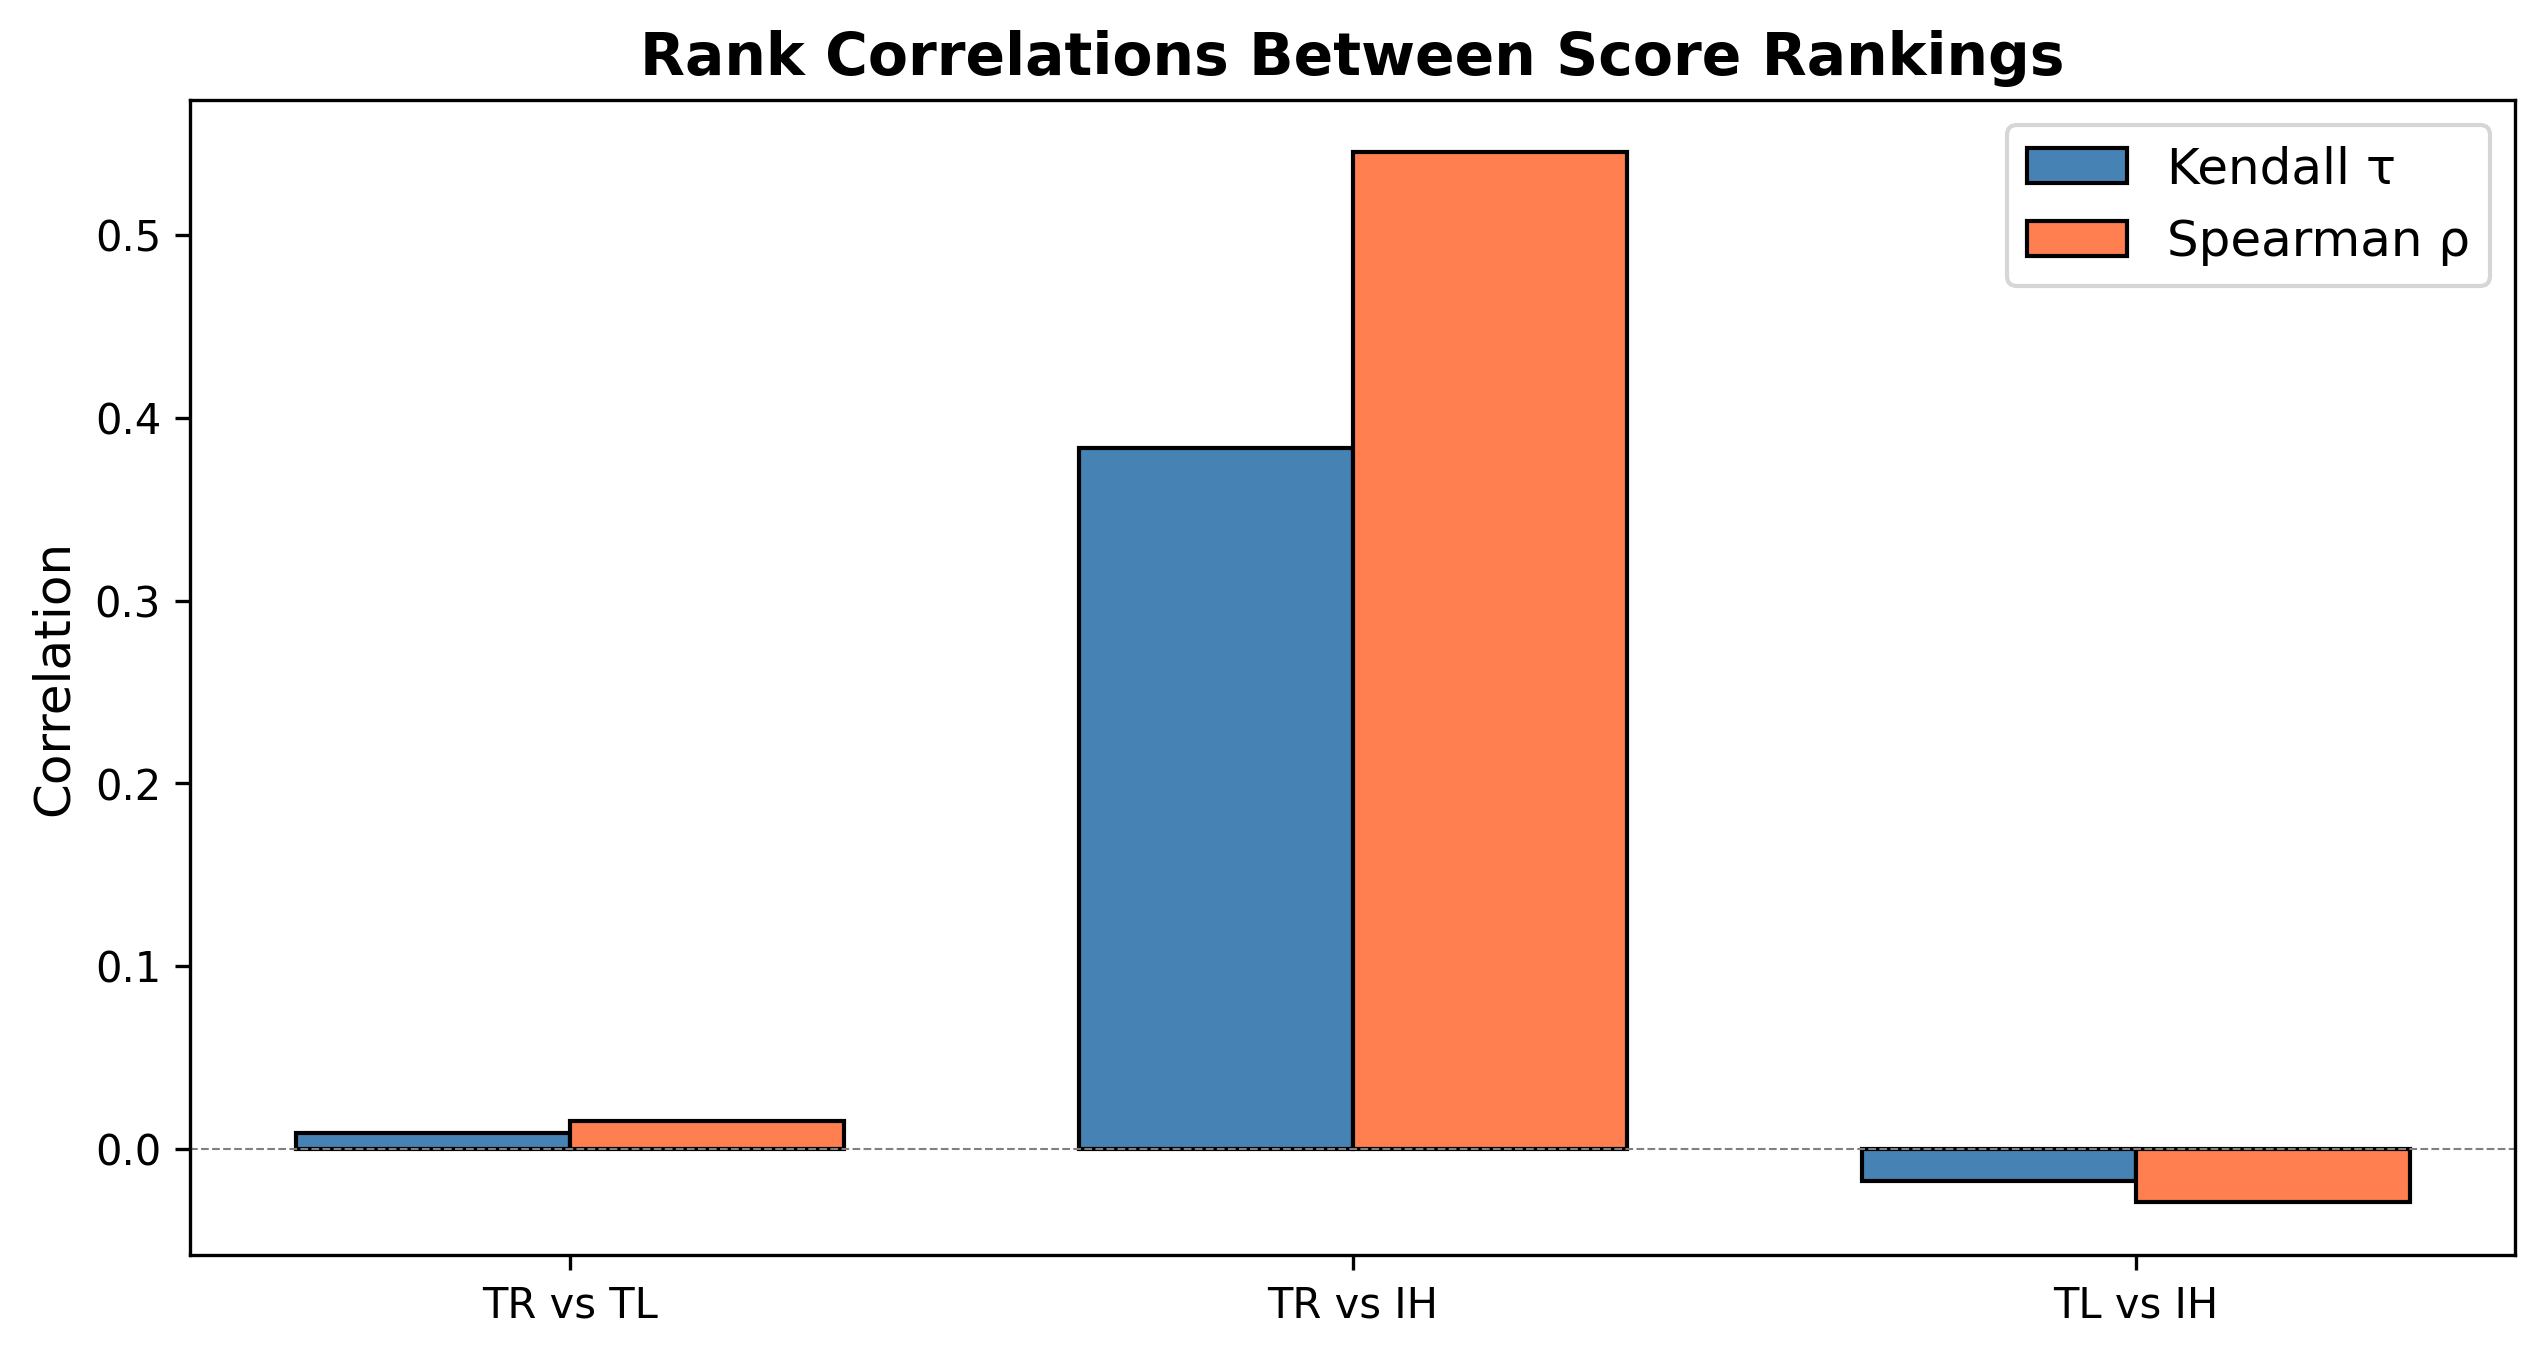
\includegraphics[width=0.32\linewidth]{assets/experiment-2-rank-correlation.png}\hfill
    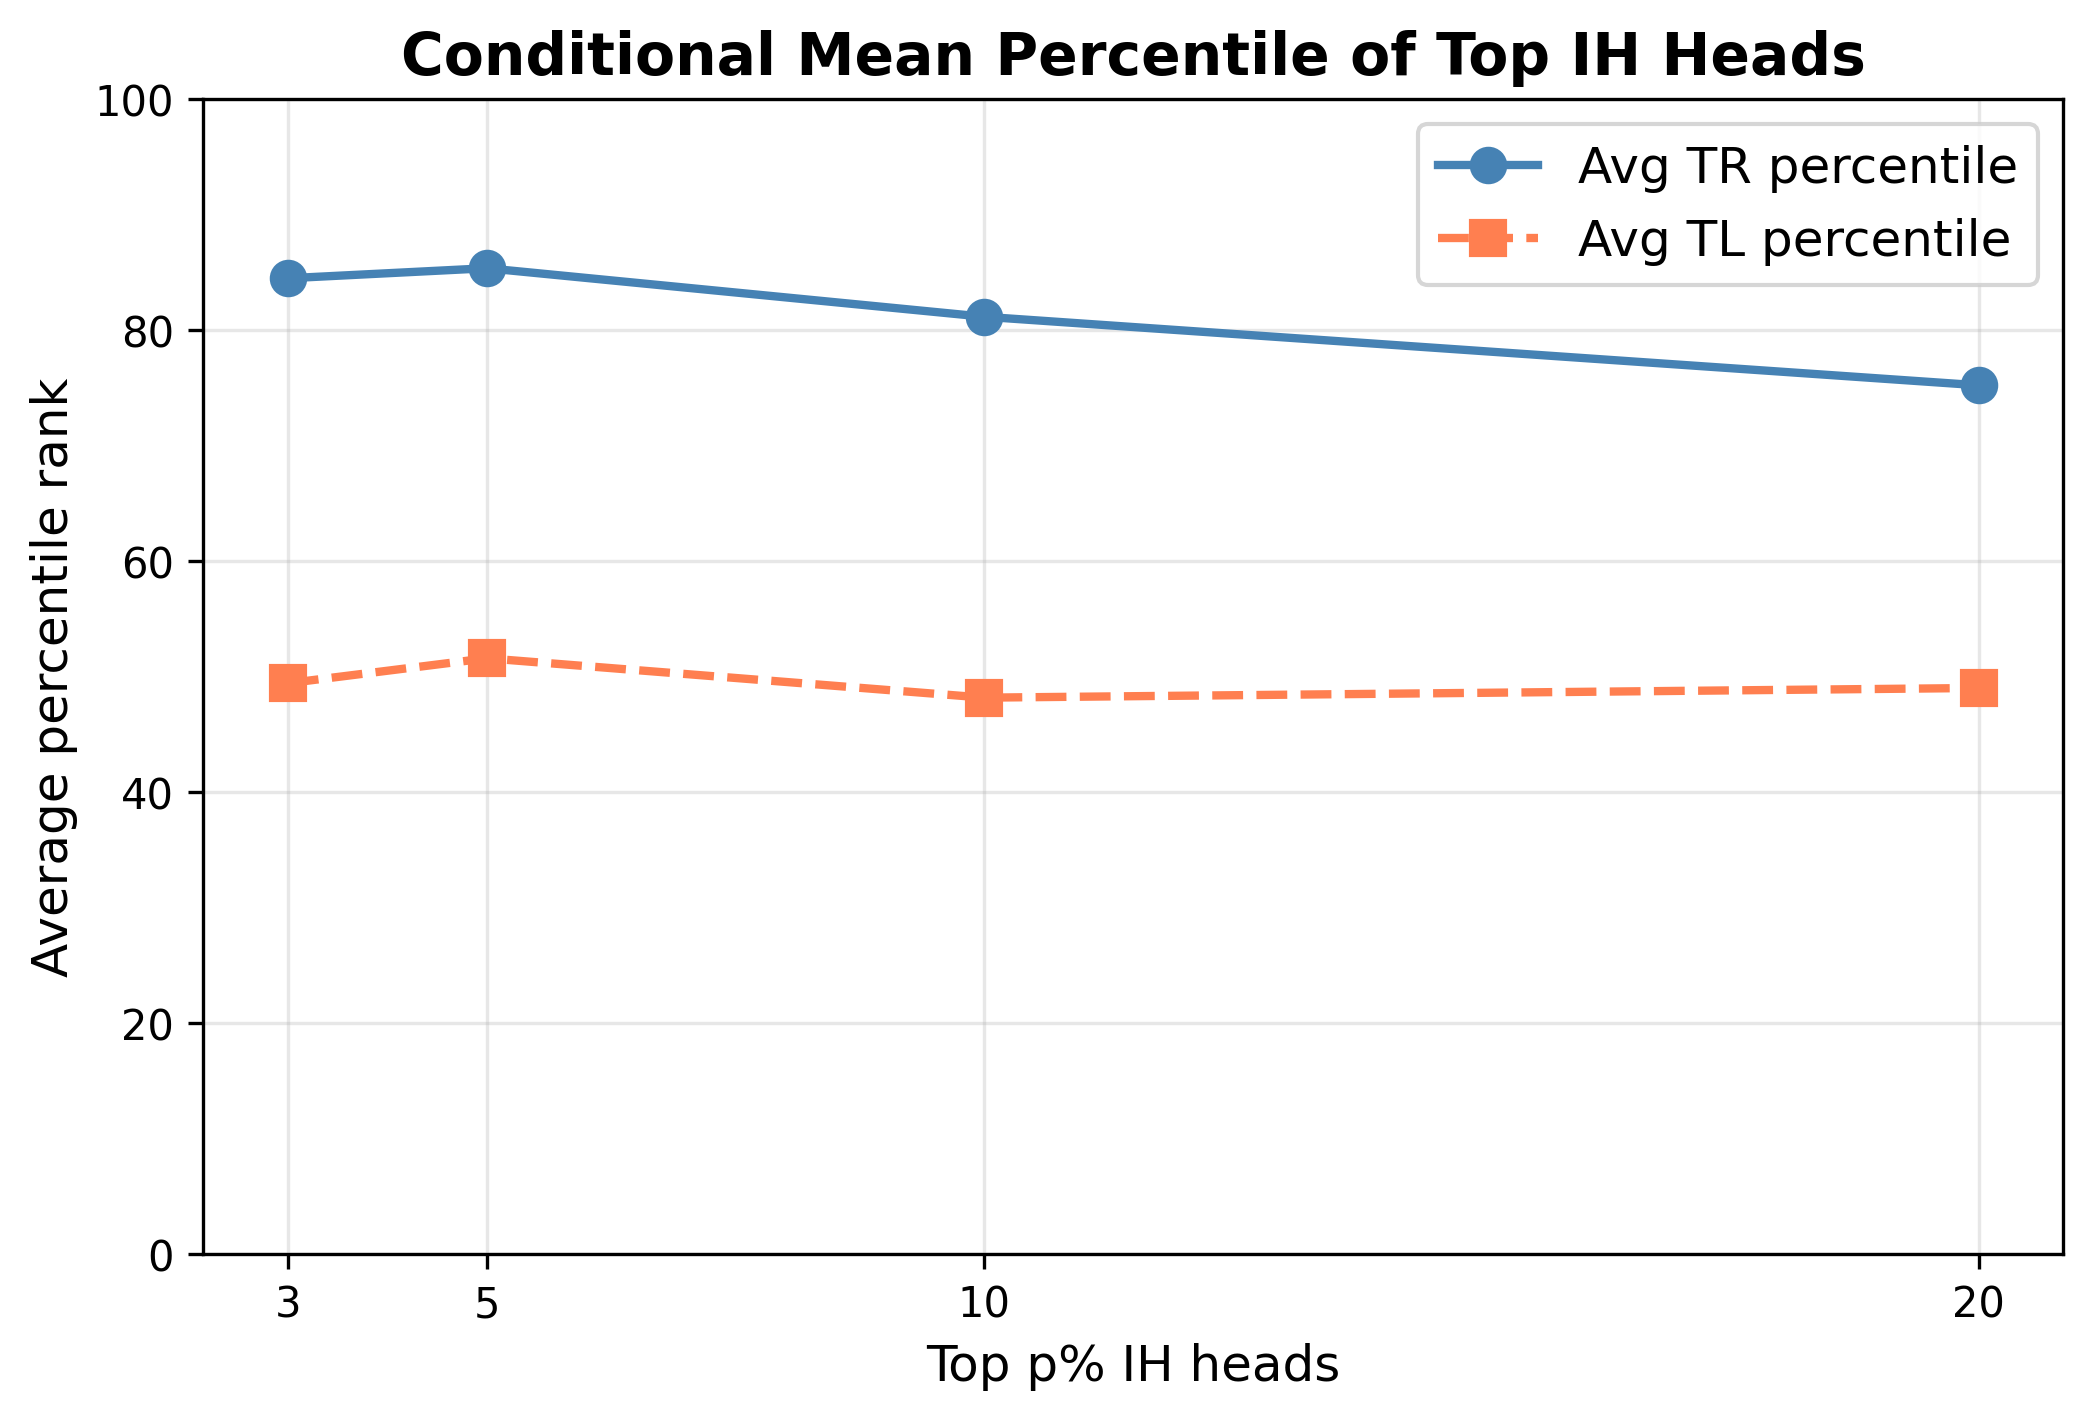
\includegraphics[width=0.32\linewidth]{assets/experiment-2-conditional-mean-percentile.png}
    \caption{Experiment 2 overlap analysis. Left: Jaccard similarity between top 3\% head sets. Center: Kendall $\tau$ and Spearman $\rho$ rank correlations across all 672 heads. Right: Conditional mean percentile analysis showing how top IH heads rank under TR vs.\ TL scores.}
    \label{fig:exp2-overlap}
\end{figure}

\subsection{Experiment 3: Ablation}

% Table: ablation results here
\begin{table}[h]
\centering
\caption{Ablation results on 200 evaluation queries. Baseline accuracy = 0.91.}
\begin{tabular}{lcc}
\toprule
\textbf{Condition} & \textbf{Accuracy} & \textbf{TR Ratio} \\
\midrule
Baseline & 0.9100 & 0.9750 \\
TR ablation & 0.8500 & 0.9150 \\
TL ablation & 0.6750 & 0.9300 \\
IH ablation & 0.5450 & 0.5650 \\
Random ablation & 0.9100 & 0.9600 \\
\bottomrule
\end{tabular}
\label{tab:ablation}
\end{table}

Several patterns emerge from Table~\ref{tab:ablation}:

\textbf{TR ablation} reduces both accuracy (91\% $\to$ 85\%) and TR ratio (97.5\% $\to$ 91.5\%). The model's overall tendency to produce valid sentiment labels decreases, consistent with the idea that TR heads steer the model into the task subspace.

\textbf{TL ablation} has a larger effect on accuracy (91\% $\to$ 67.5\%) while TR ratio stays high (93\%). This pattern is consistent with the paper's prediction: the model still ``knows'' it is doing sentiment classification (high TR ratio), but it picks the wrong label more often without TL heads.

\textbf{IH ablation} is the most damaging: accuracy drops to 54.5\% (near chance for binary) and TR ratio collapses to 56.5\%. This makes sense, since induction heads implement the copying mechanism that both TR and TL rely on. Disabling them disrupts the entire ICL pipeline.

\textbf{Random ablation} has essentially zero effect (accuracy unchanged at 91\%), confirming that the observed degradations are specific to the functional head sets, not an artifact of removing any 20 heads.

\begin{figure}[h!]
    \centering
    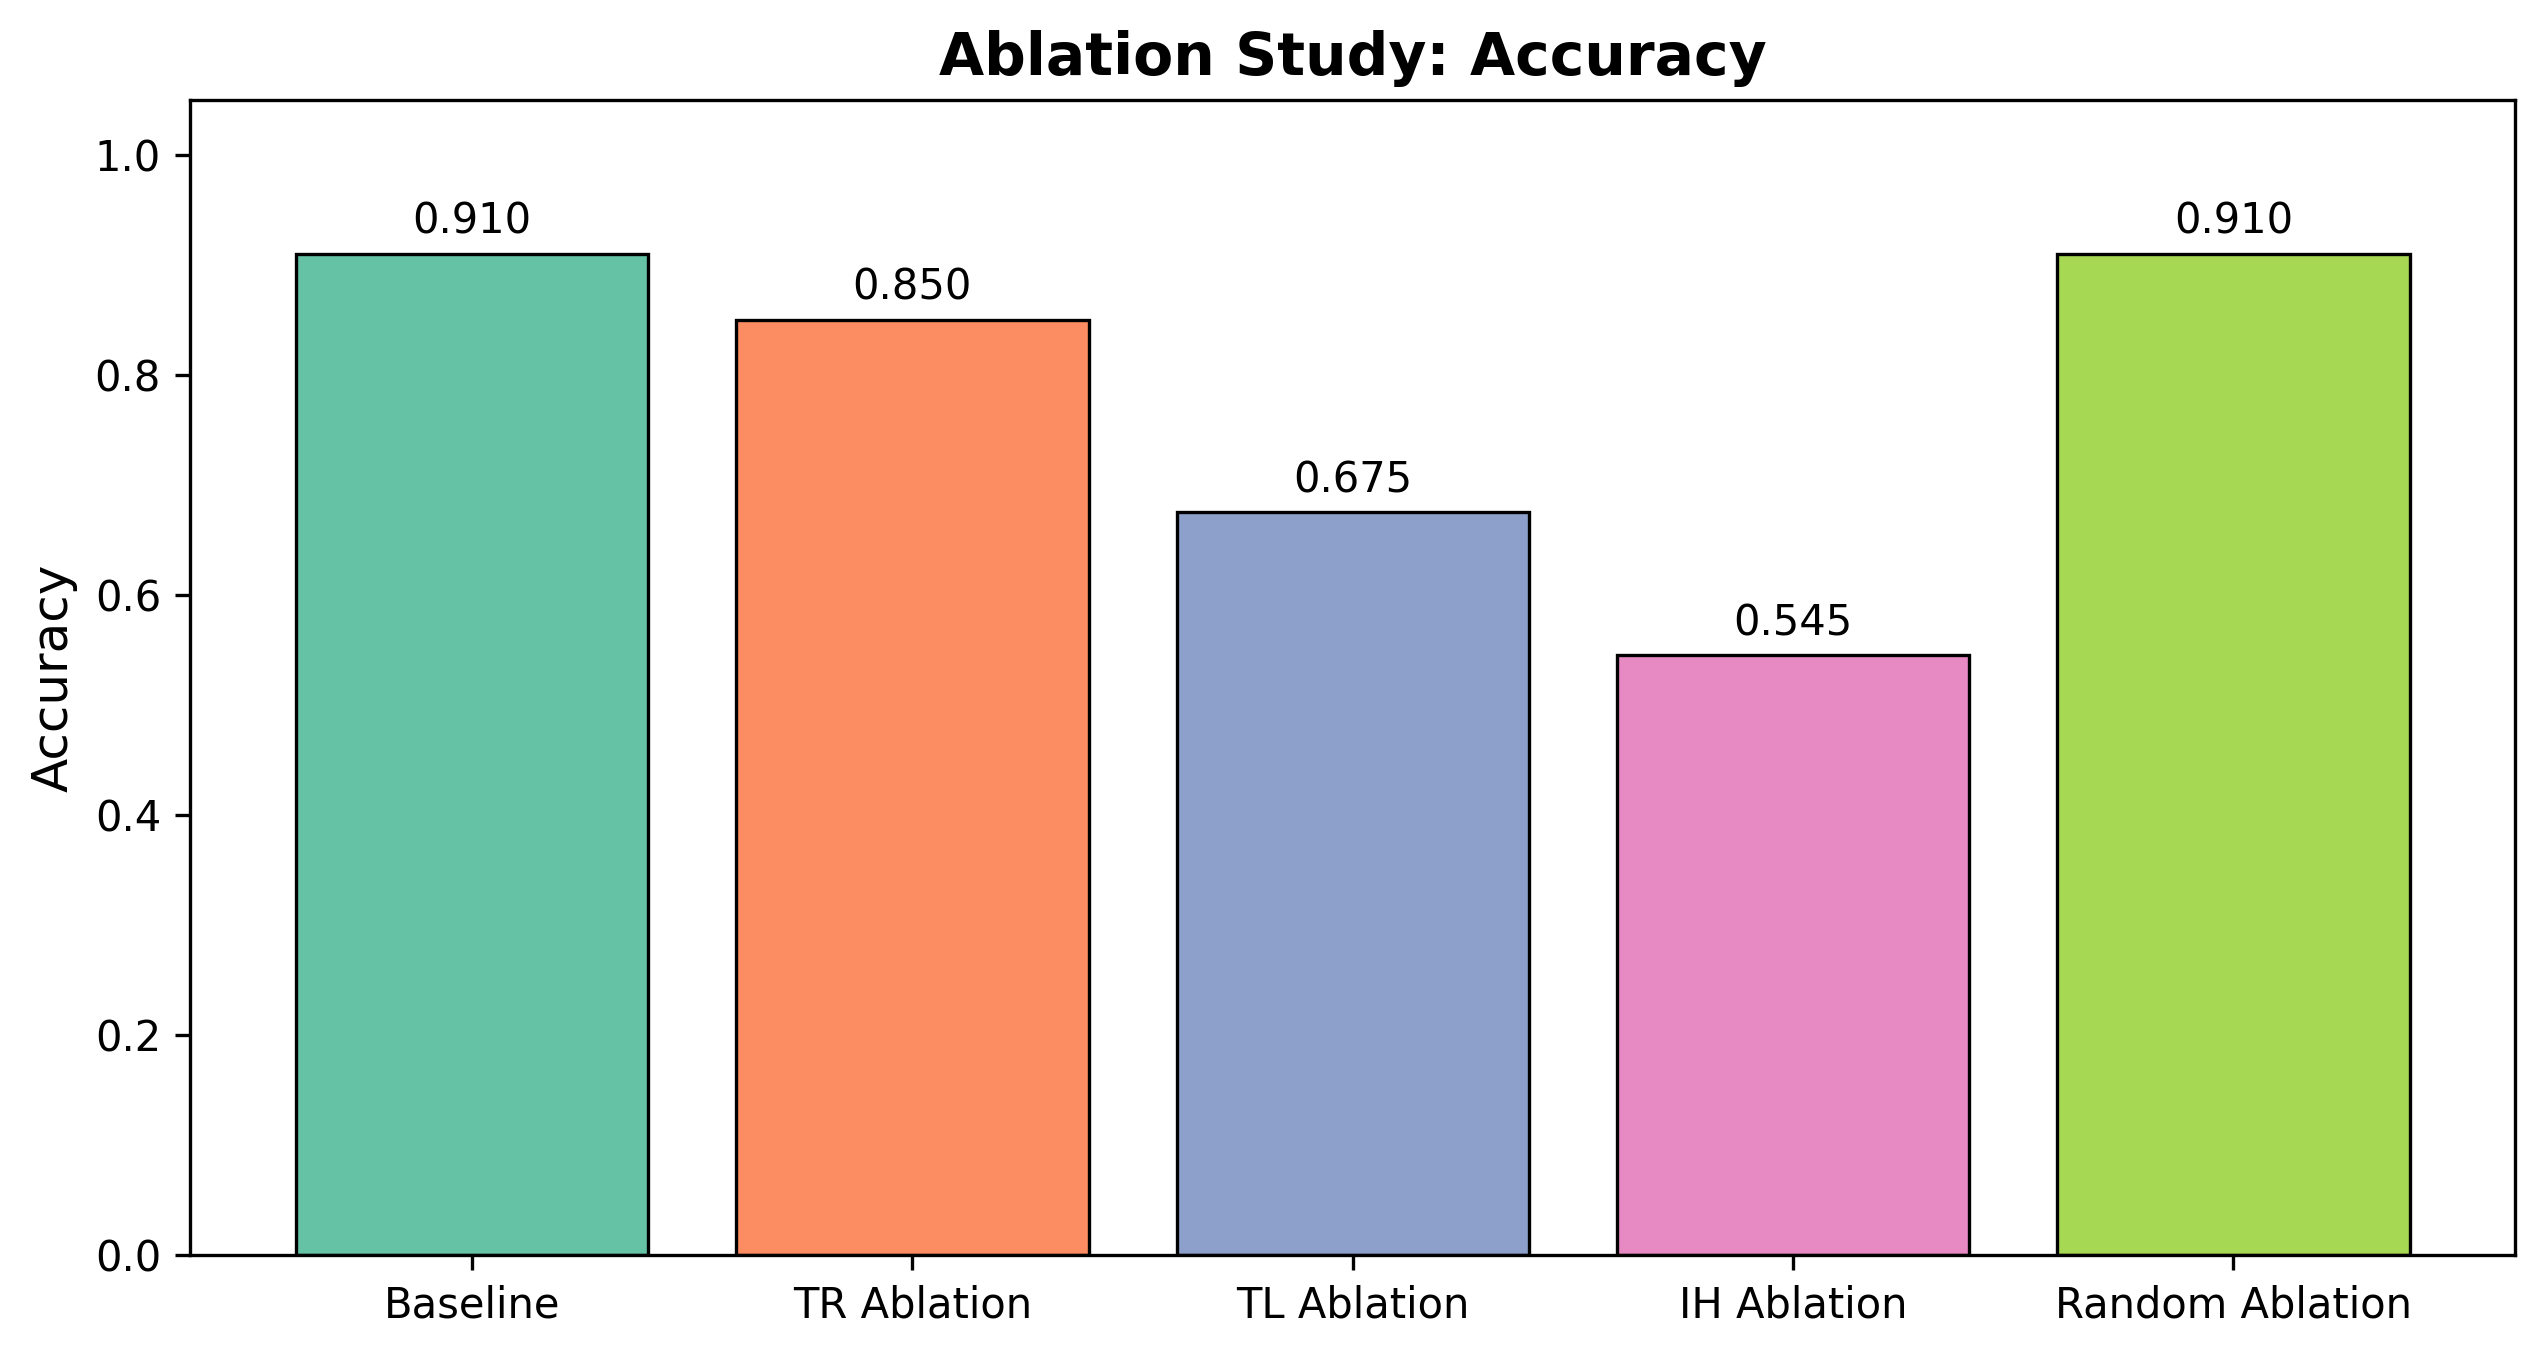
\includegraphics[width=0.48\linewidth]{assets/experiment-3-abalation-accuracy.png}\hfill
    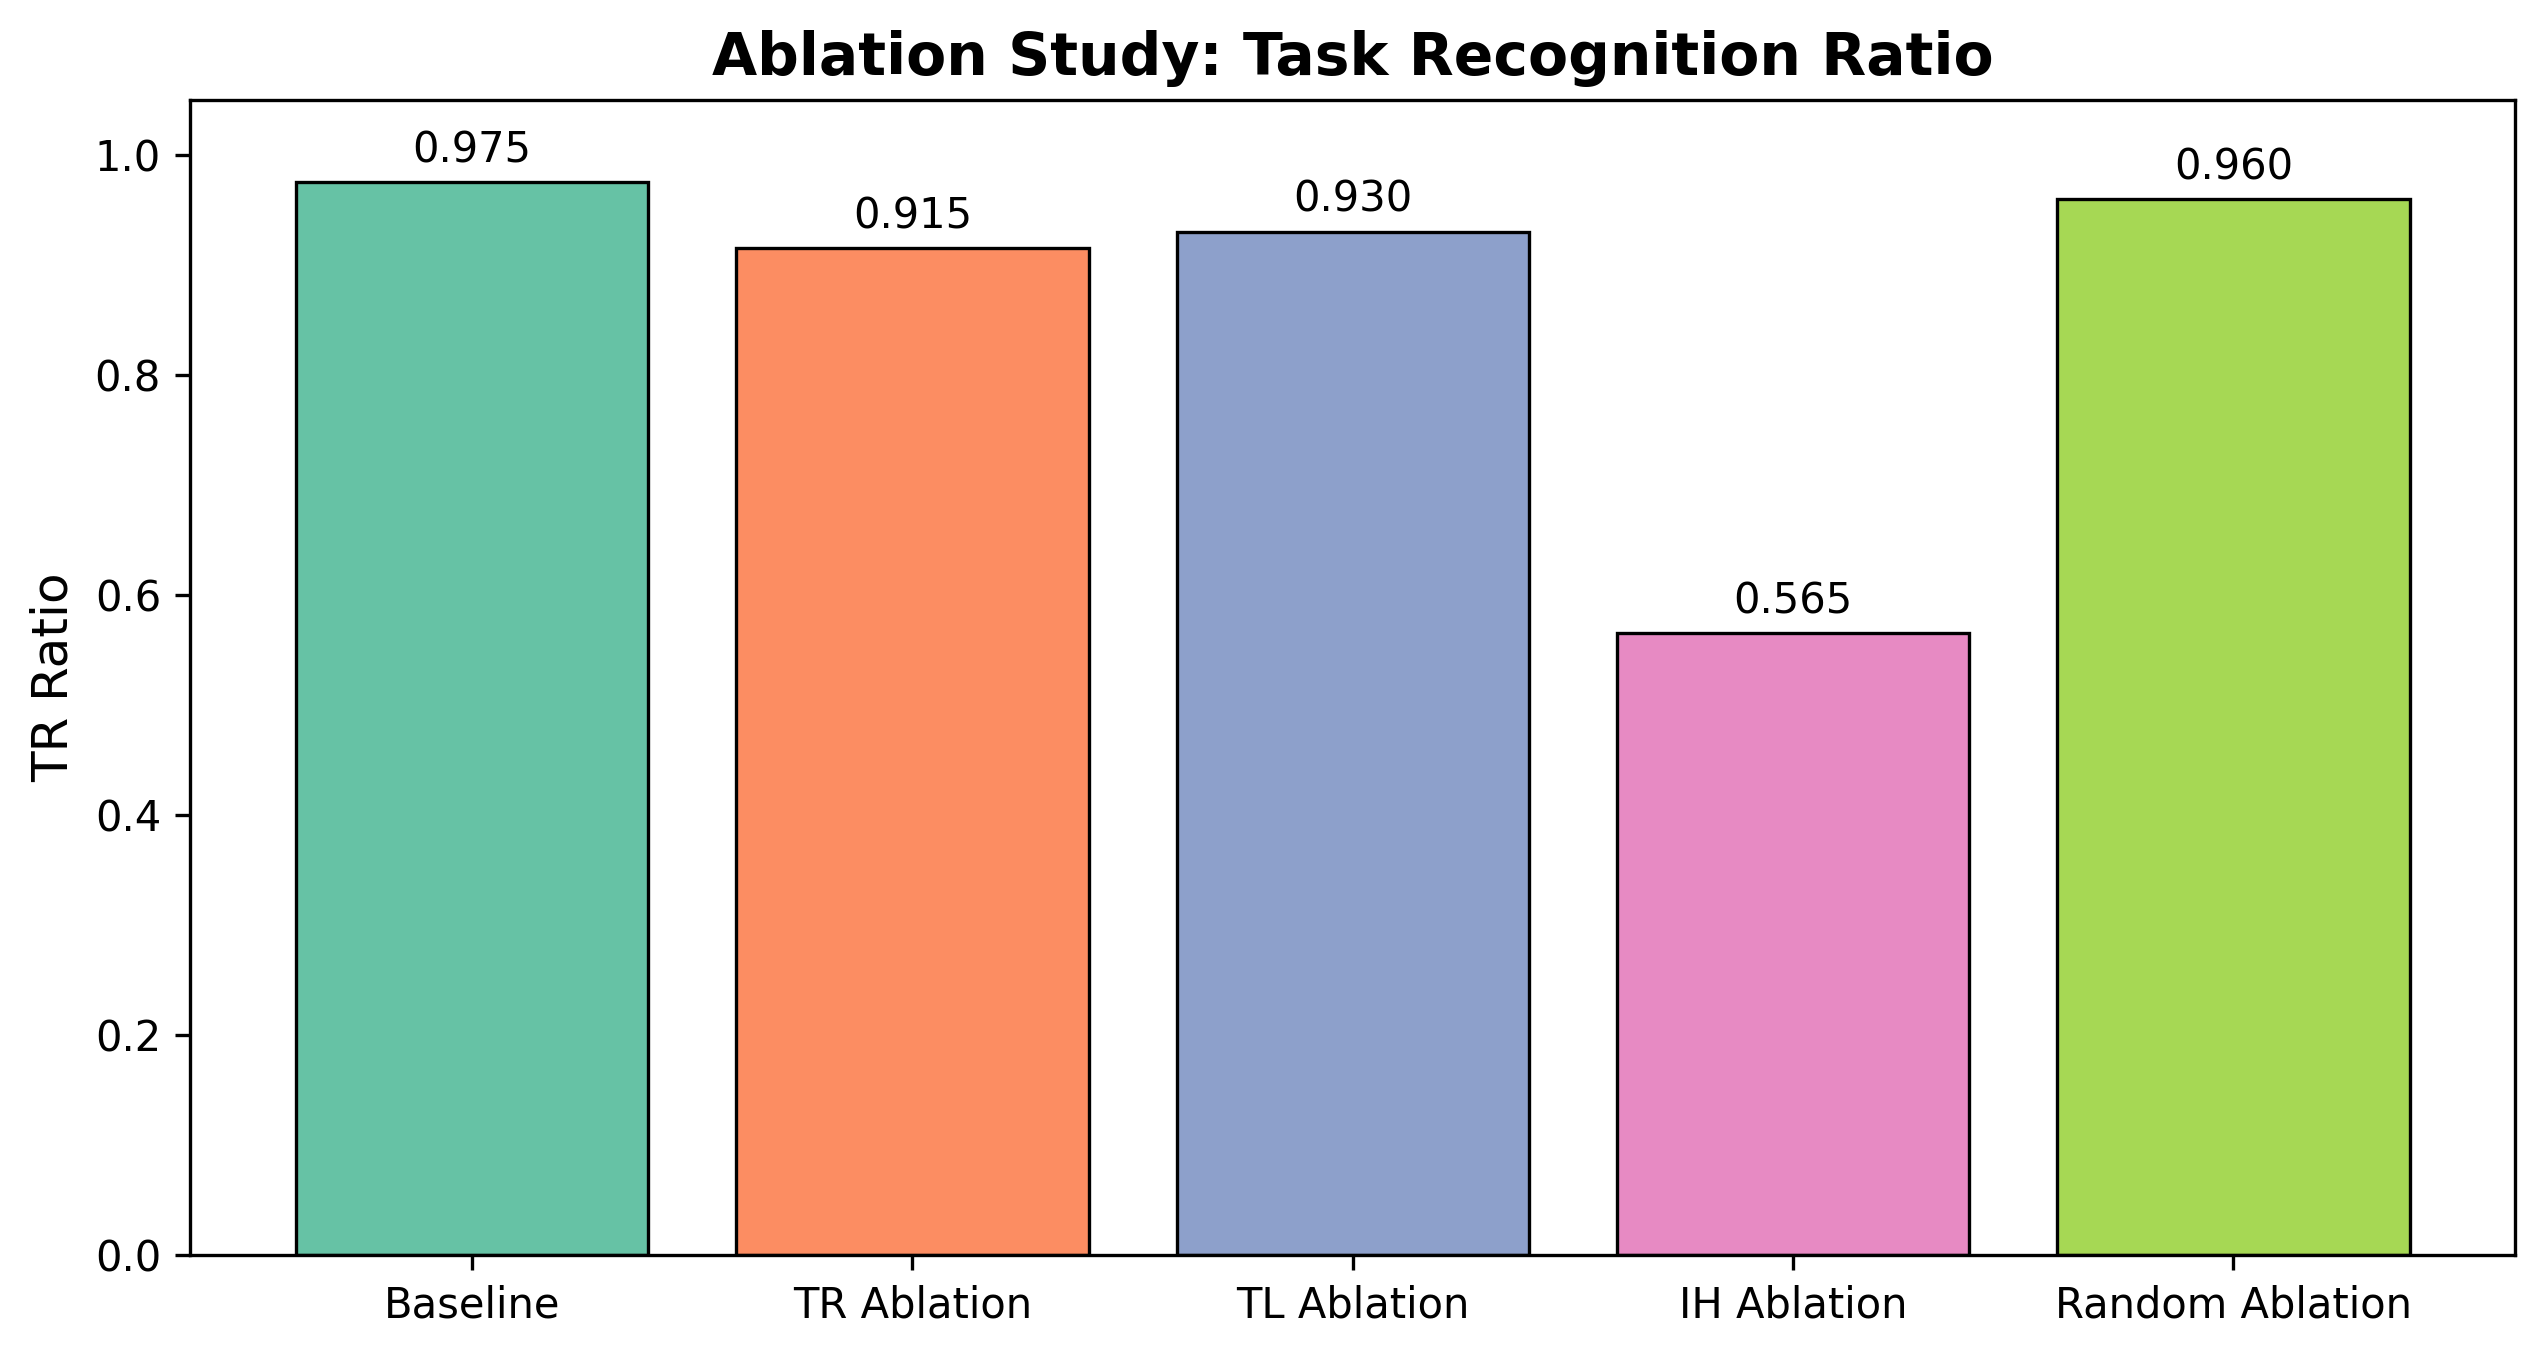
\includegraphics[width=0.48\linewidth]{assets/experiment-3-tr-ration.png}
    \caption{Experiment 3 ablation results. Left: Accuracy under each ablation condition. Right: TR ratio (fraction of predictions mapping to a valid task label) under each ablation condition. TL ablation sharply reduces accuracy while preserving TR ratio; IH ablation degrades both.}
    \label{fig:exp3-ablation}
\end{figure}


\subsection{Experiment 4: Layer-wise Distribution}

% Table: layer distribution here
\begin{table}[h]
\centering
\caption{Layer distribution statistics for top 3\% head sets.}
\begin{tabular}{lccc}
\toprule
\textbf{Head Type} & \textbf{Mean Layer} & \textbf{Median Layer} & \textbf{Std} \\
\midrule
TR & 22.65 & 24.0 & 5.18 \\
TL & 14.95 & 15.5 & 6.93 \\
IH & 14.90 & 14.5 & 5.94 \\
Random & 13.65 & 13.0 & 8.94 \\
\bottomrule
\end{tabular}
\label{tab:layers}
\end{table}

TR heads are concentrated in the \textbf{deepest layers}, with a mean layer index of 22.65 out of 28 (Table~\ref{tab:layers}). TL and IH heads cluster around layers 14--15, in the middle of the network, with nearly identical means (14.95 vs.\ 14.90).

Mann-Whitney U tests confirm these differences are statistically significant: TL vs.\ TR yields $p = 3.2 \times 10^{-5}$, IH vs.\ TR yields $p = 1.9 \times 10^{-4}$, while TL vs.\ IH is not significant ($p = 0.56$). This pattern (TR deep, TL and IH in the middle, TL $\approx$ IH) is consistent with the paper's findings.

So the model first attends to demonstration labels and builds intermediate representations (IH and TL in middle layers), and then deeper heads project those representations into the label subspace (TR in late layers).


\begin{figure}[h!]
    \centering
    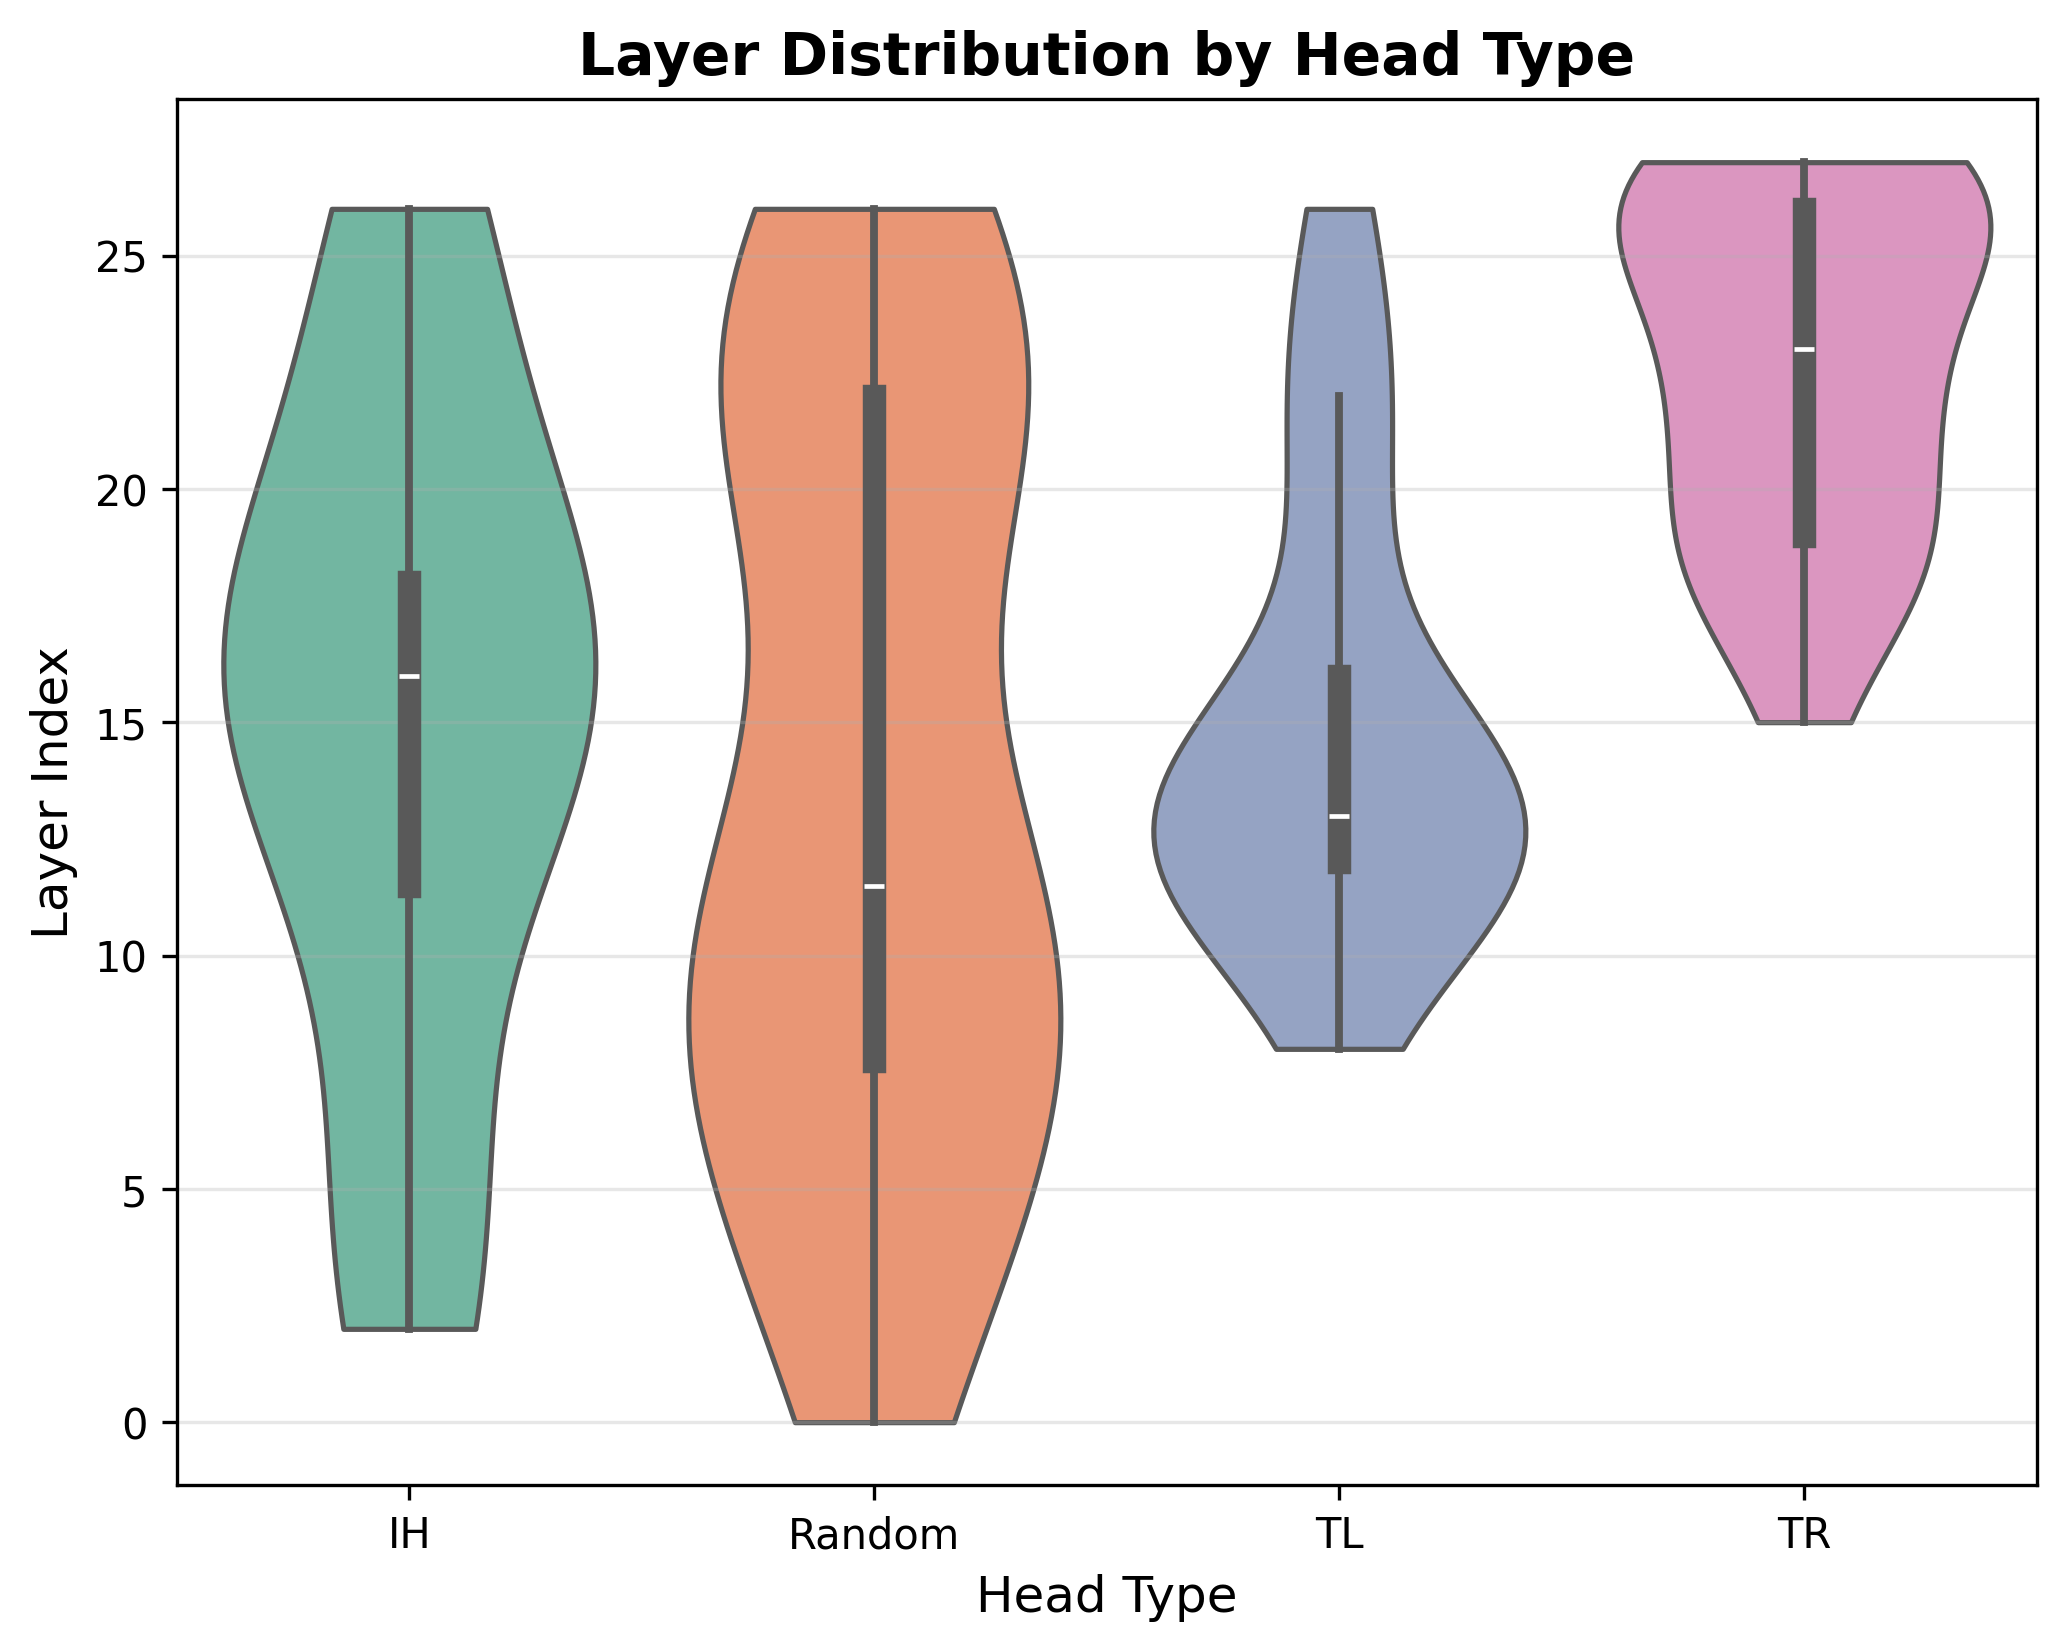
\includegraphics[width=0.48\linewidth]{assets/experiment-4-violin -plot.png}\hfill
    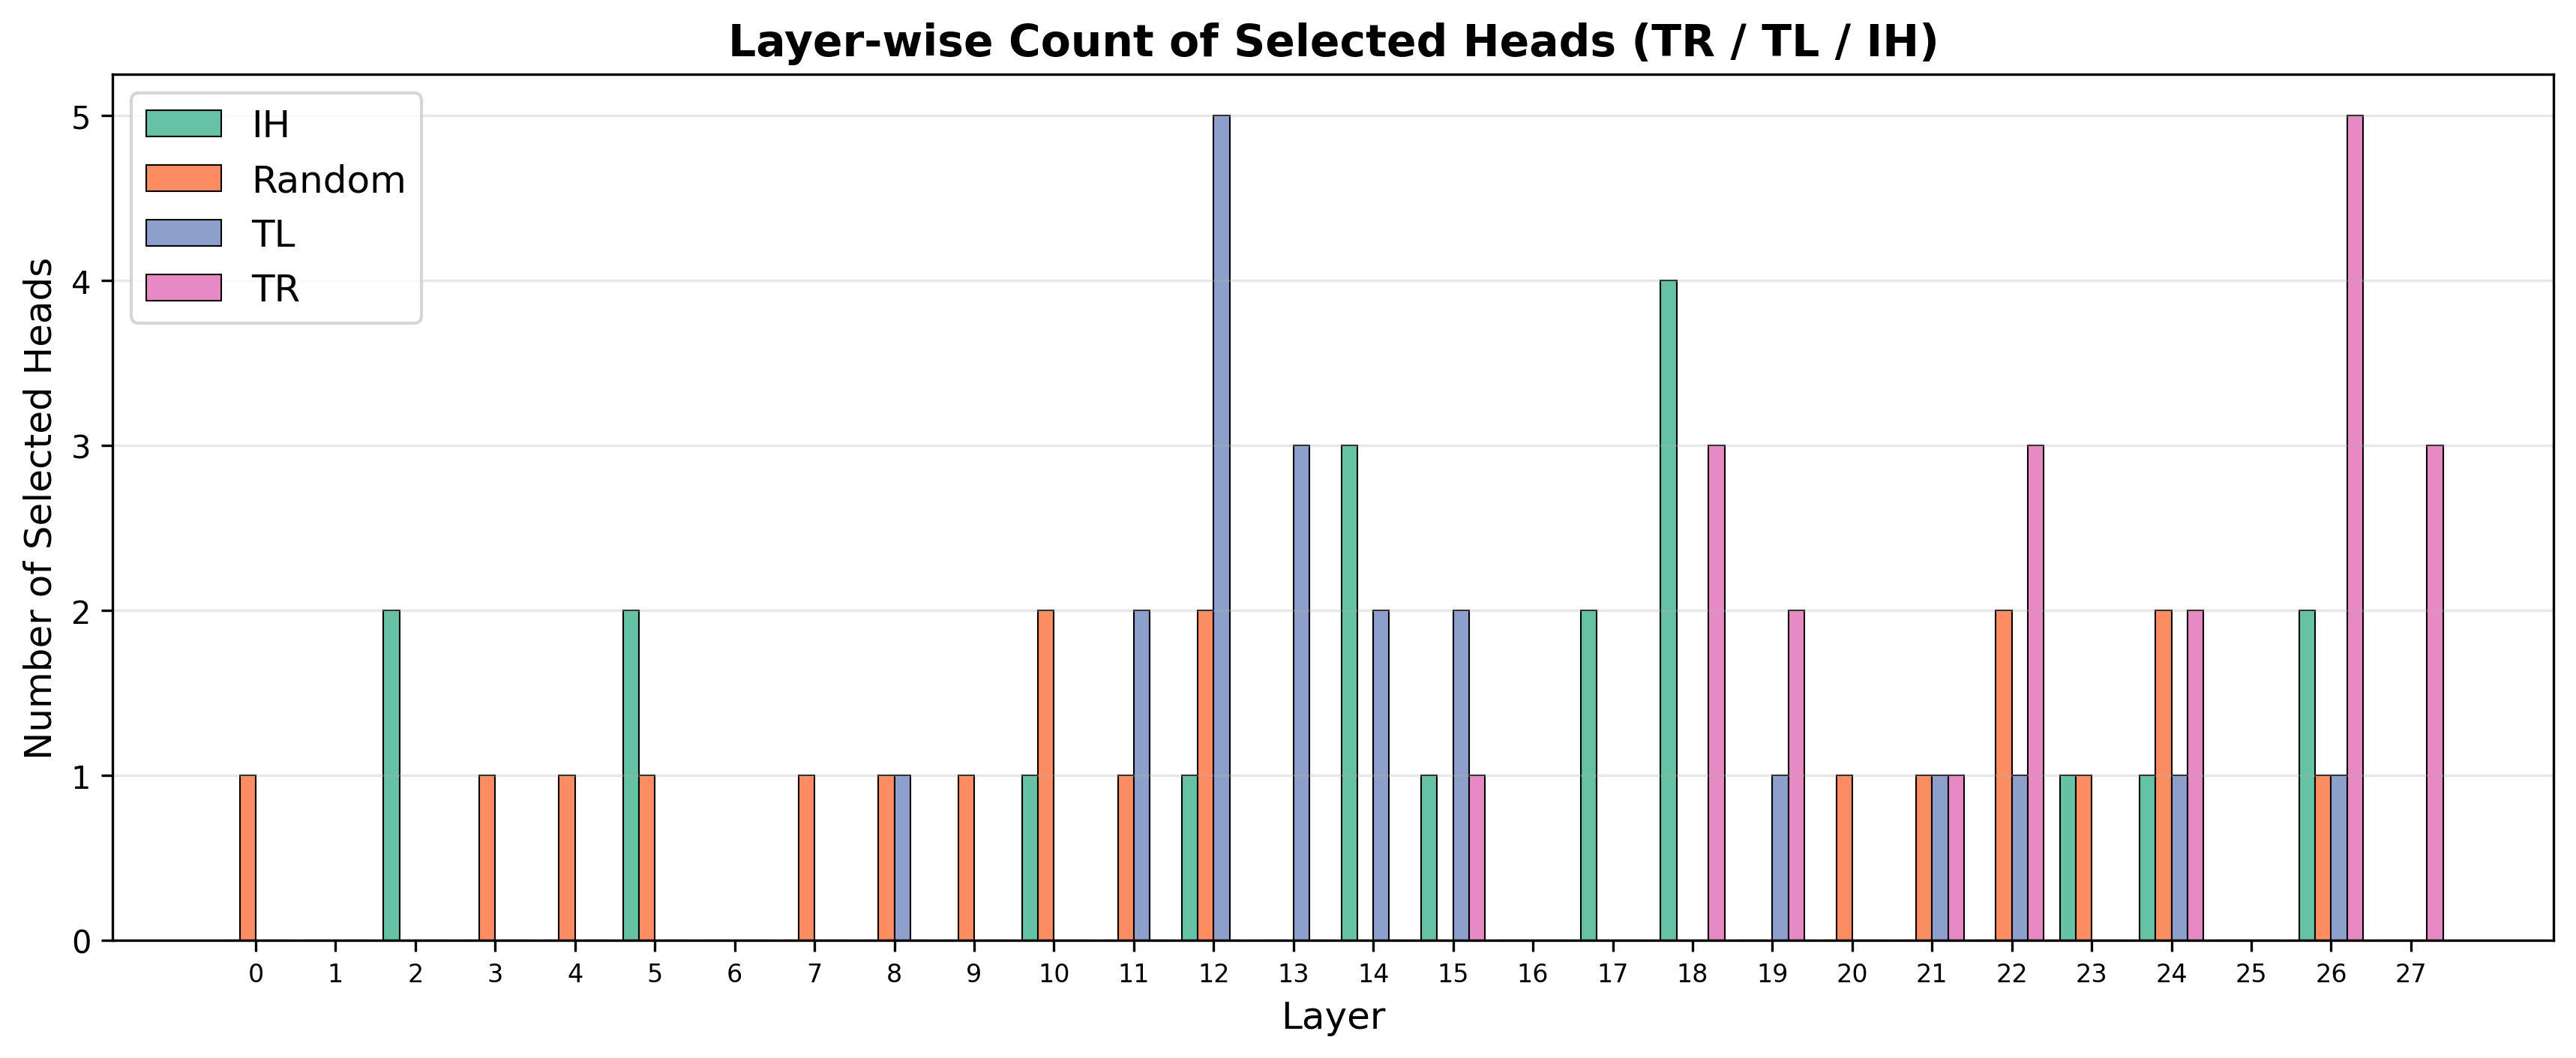
\includegraphics[width=0.48\linewidth]{assets/experiment-4-layer-count.png}
    \caption{Experiment 4 layer-wise distribution of head types. Left: Violin plot showing the distribution of layer indices for each head set. TR heads cluster in the deepest layers (mean $\approx$ 23), while TL and IH heads concentrate around layers 14--15. Right: Per-layer head counts for each type.}
    \label{fig:exp4-layers}
\end{figure}

\subsection{Experiment 5: Attention Distribution}

% Table: attention distribution here
\begin{table}[h]
\centering
\caption{Mean attention allocation from query prediction position to different token groups.}
\begin{tabular}{lcc}
\toprule
\textbf{Head Type} & \textbf{Demo Labels} & \textbf{Query Tokens} \\
\midrule
TR & 0.3044 & 0.0218 \\
TL & 0.0739 & 0.3325 \\
IH & 0.6987 & 0.0057 \\
Random & 0.0823 & 0.0985 \\
\bottomrule
\end{tabular}
\label{tab:attention}
\end{table}

The attention allocation patterns (Table~\ref{tab:attention}) are remarkably clean. IH heads devote nearly 70\% of their attention to demo-label tokens, consistent with their role as ``copy from previous labels'' heads. TR heads also show elevated demo-label attention (30\%) compared to random (8\%), suggesting they partially rely on similar positional cues.

TL heads show the opposite pattern: 33\% of attention goes to query-sentence tokens, with minimal attention to demo labels (7\%). This supports the interpretation that TL heads are processing the query content to determine the correct answer, rather than attending to demonstration structure.

Random heads split their attention roughly evenly across the prompt with no structured pattern, serving as a useful null baseline.

\begin{figure}[h!]
    \centering
    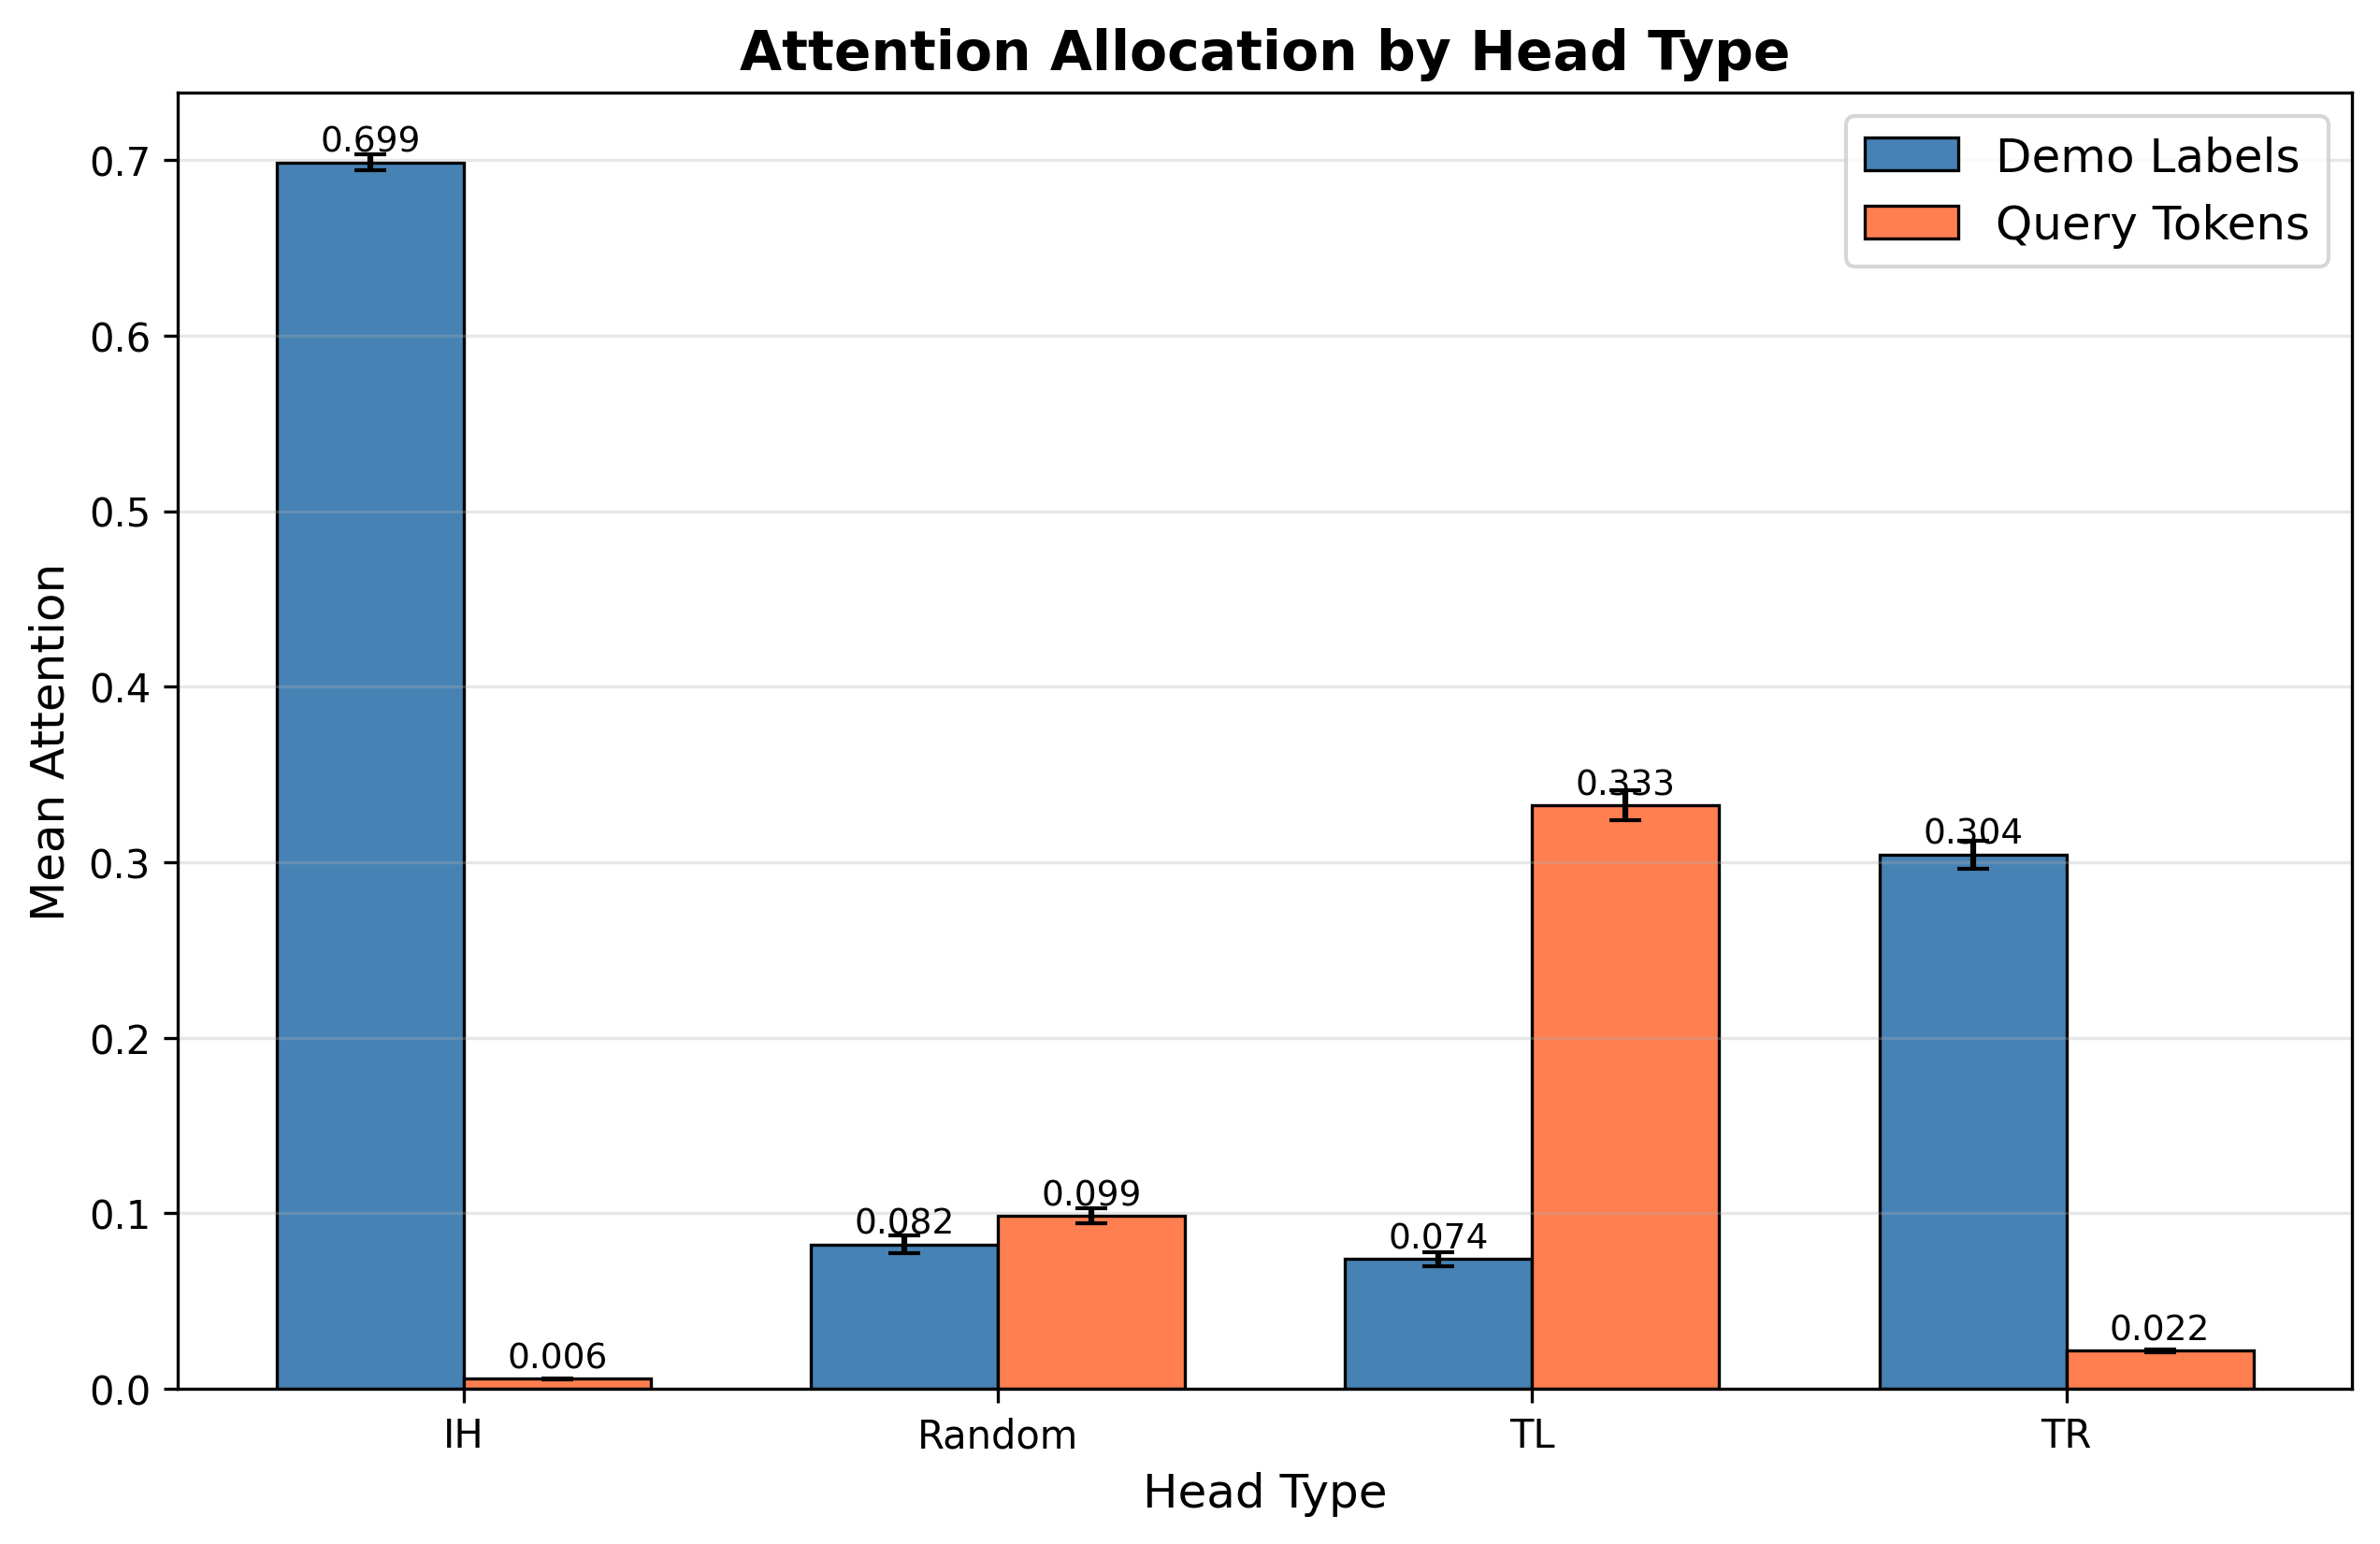
\includegraphics[width=0.48\linewidth]{assets/experiment-5-attention-allocation.png}\hfill
    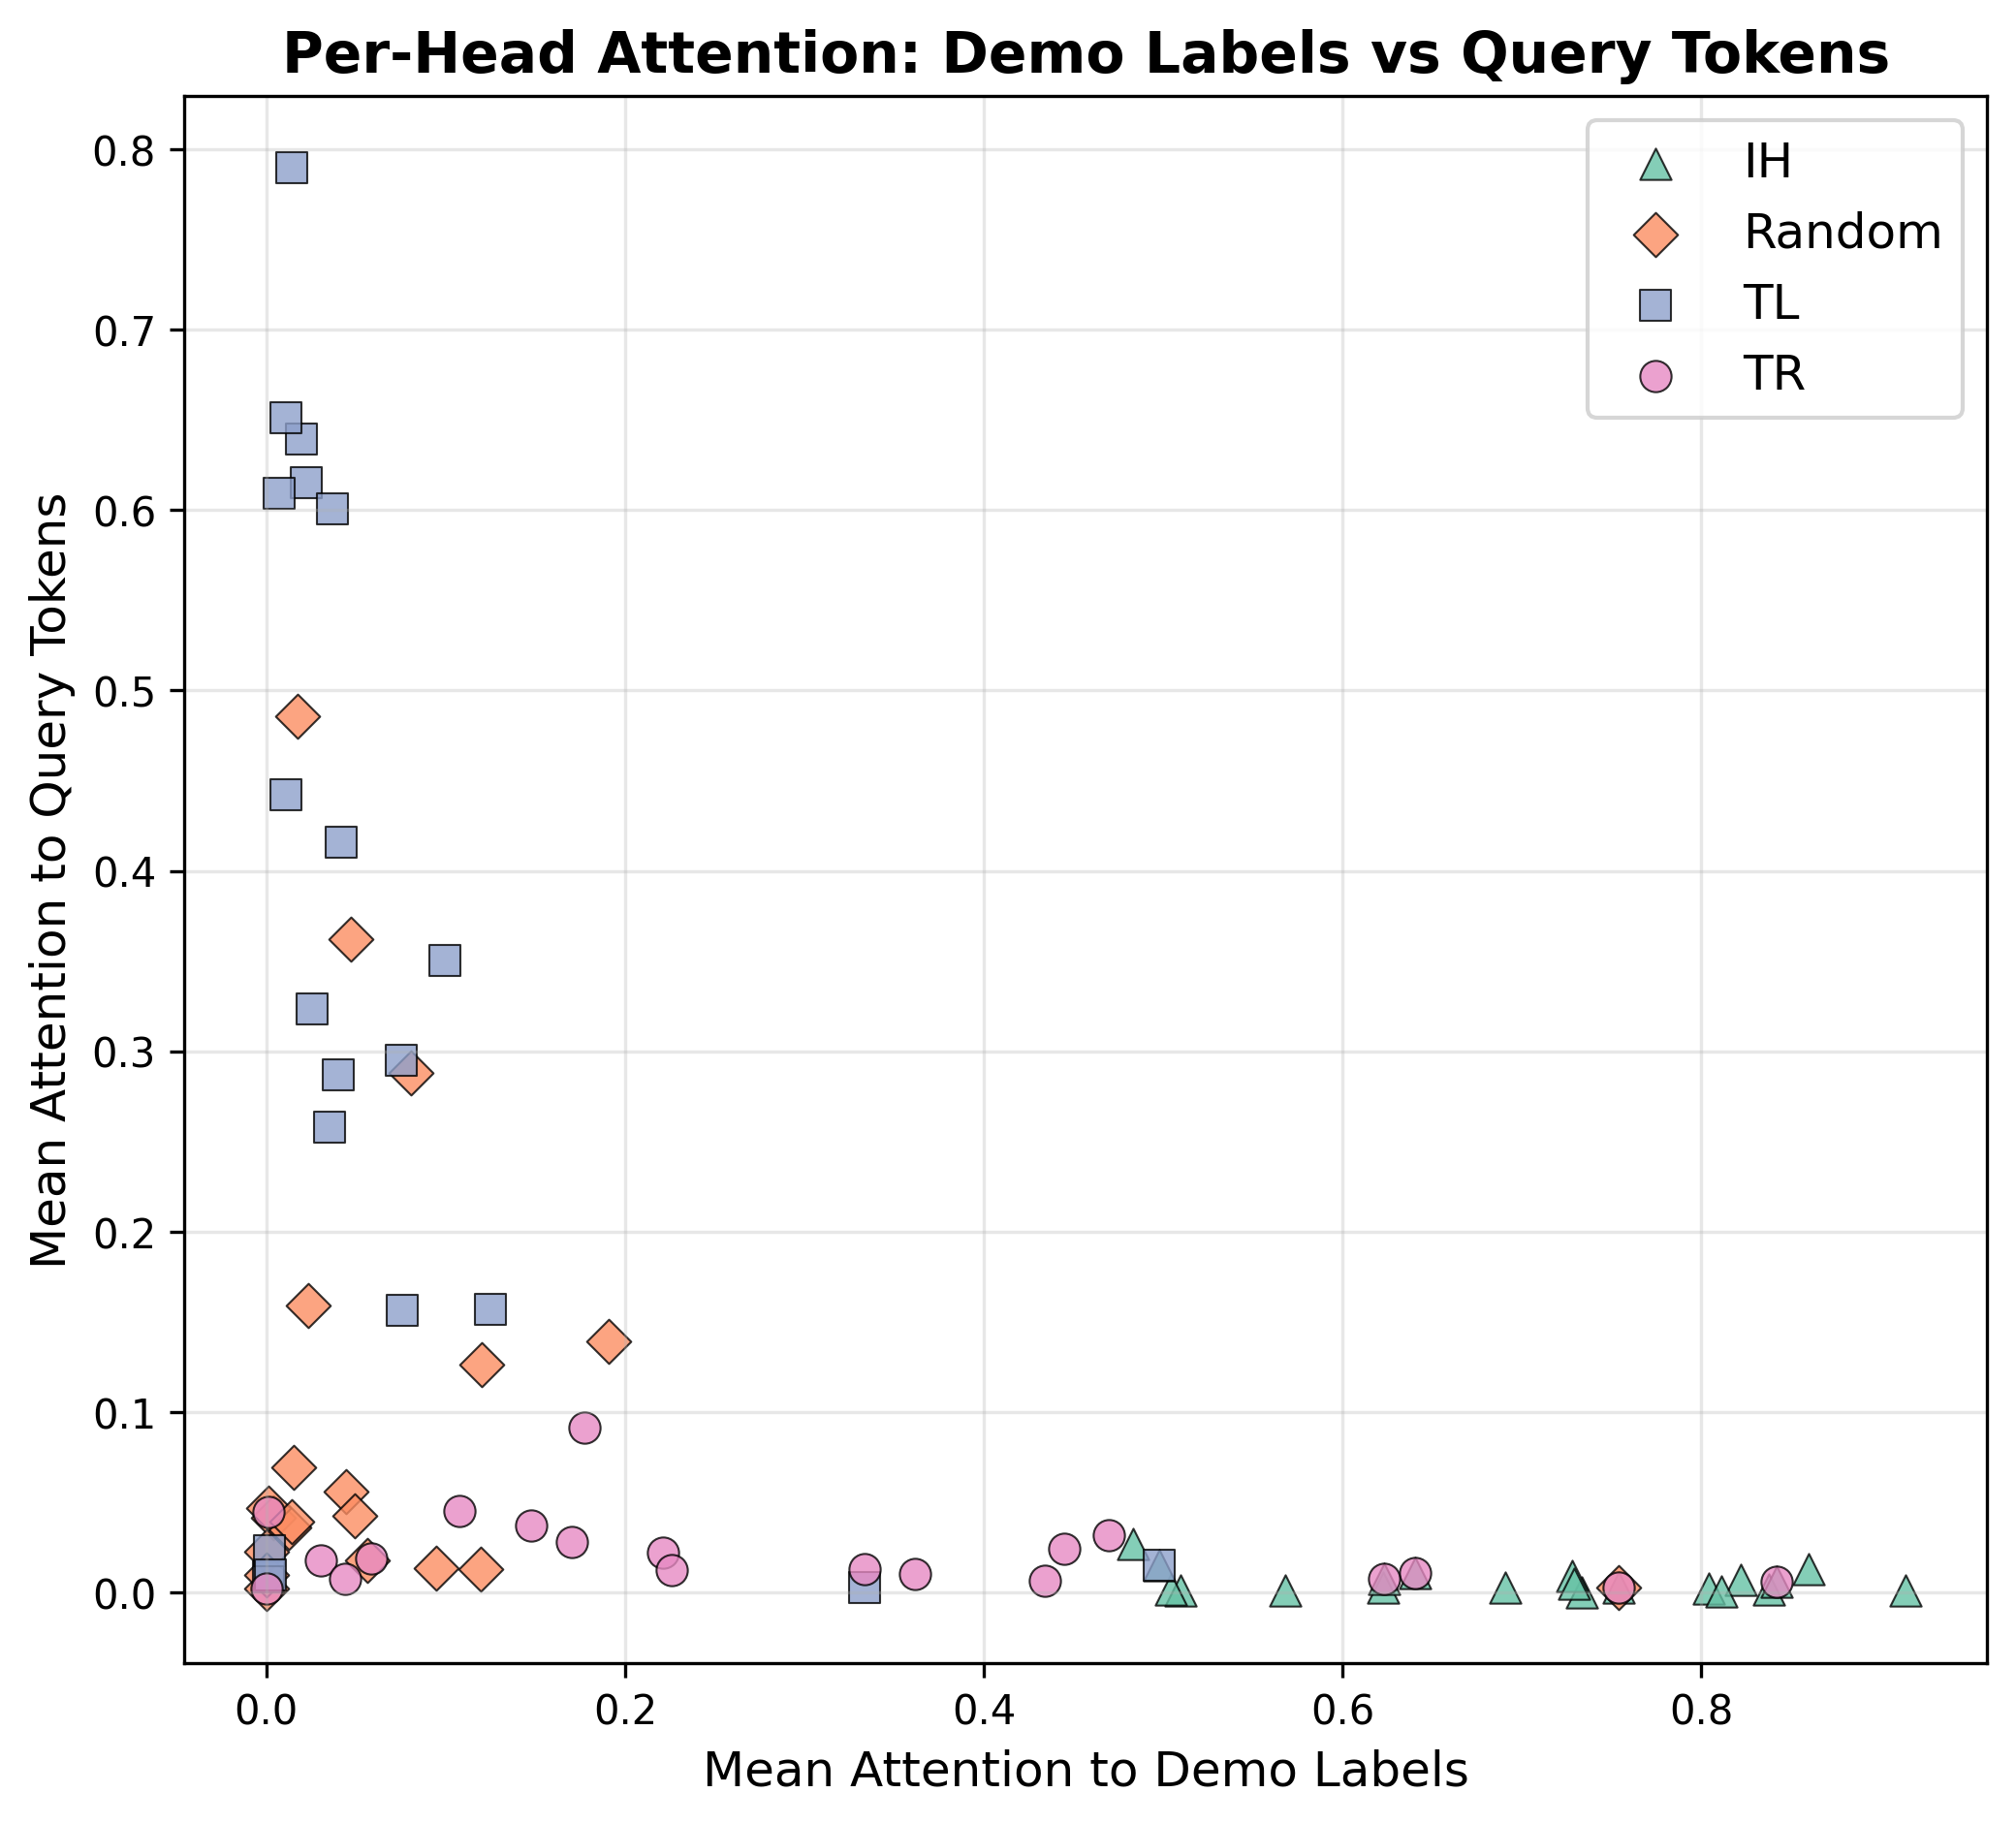
\includegraphics[width=0.48\linewidth]{assets/experiment-5-scatter.png}
    \caption{Experiment 5 attention distribution analysis. Left: Grouped bar chart of mean attention allocation to demo-label and query-sentence tokens by head type. Right: Scatter plot of demo-label vs.\ query-token attention for individual heads, colored by type.}
    \label{fig:exp5-attention}
\end{figure}

\subsection{Discussion}

Taking all five experiments together, the results paint a consistent picture: TR and TL heads are functionally and structurally distinct components that perform separable sub-computations during in-context learning.

The most compelling evidence comes from the \textbf{convergence of independent measurements}. TR heads are identified by their projection onto the task subspace (Exp.\ 1), yet they independently turn out to be (a) correlated with induction heads (Exp.\ 2), (b) concentrated in deeper layers (Exp.\ 4), and (c) disproportionately attending to demo labels (Exp.\ 5). These properties were not used in their selection; they emerge from the analysis.

The IH ablation result (Exp.\ 3) is worth highlighting: it produced the largest performance drop across all conditions. This suggests that induction heads may be a shared substrate that both TR and TL computations depend on, rather than belonging exclusively to one category.

% ============================================================================
% 11. LIMITATIONS
% ============================================================================
\section{Limitations} \label{sec:limitations}

\begin{itemize}
    \item \textbf{Single dataset.} All experiments use SST-2 only. The paper tests on multiple tasks (NLI, topic classification, etc.), and it is possible that some findings are task-specific.
    \item \textbf{Single model.} We use one model architecture (Llama-3.2-3B). The original paper tests on six models spanning three architecture families (Llama, Qwen, Yi) and sizes from 3B to 34B; cross-architecture generalization is not tested here.
    \item \textbf{No multi-token labels.} Our label words (``positive,'' ``negative'') tokenize to single tokens, so we do not test the multi-token case.
\end{itemize}

% ============================================================================
% 12. PLAN FOR END-TERM ASSESSMENT
% ============================================================================
\section{Plan for End-term Assessment} \label{sec:endterm}

\begin{enumerate}
    \item \textbf{Multi-task generalization.} Extend the analysis to at least two additional tasks (e.g., AG News for topic classification, RTE or MNLI for natural language inference) to test whether the TR/TL separation is task-general or SST-2-specific.
    \item \textbf{Varying $n$-shot.} Investigate how TR and TL head sets change with the number of demonstrations (e.g., 2-shot, 4-shot, 16-shot). The hypothesis is that TR heads should be more stable across $n$-shot settings than TL heads.
    \item \textbf{Targeted ablation refinement.} Instead of zeroing entire heads, try partial ablation (scaling head outputs by a factor $< 1$) or ablating only the task-subspace component of a head's output to test more specific causal claims.
    \item \textbf{Extending TSLA beyond single-position localization.} A promising direction for the end-term project is to generalize TSLA from a single prediction position to a \emph{multi-position} setting. The current paper identifies TR and TL heads using head outputs at one final position, and the authors themselves note that this becomes limiting in composite prompts, where the learned task vectors help mainly for the first subtask. I will try to define multi-position TR/TL score.
\end{enumerate}

% ============================================================================
% 13. CONCLUSION
% ============================================================================
\section{Conclusion} \label{sec:conclusion}

We reproduced the core findings of \cite{TSLA} on SST-2 using \texttt{unsloth/Llama-3.2-3B-Instruct-bnb-4bit} with 8-shot in-context learning. Across five experiments, we found robust evidence for the separation of task recognition and task learning into distinct attention head populations. TR heads overlap with induction heads, reside in deeper layers, and attend to demonstration labels. TL heads are disjoint from TR heads, occupy middle layers, and attend to query content. Ablating each head set produces distinct degradation patterns consistent with their proposed functional roles. These results hold qualitatively despite a smaller model, 4-bit quantization, and a single-task setup, suggesting that the TR/TL decomposition is a robust structural feature of how transformers implement in-context learning.

% ============================================================================
% REFERENCES
% ============================================================================
\section{References} \label{sec:references}

\begin{thebibliography}{9}

\bibitem{TSLA}
Yang, H., Cho, H., and Inoue, N.\ (2025).
``Localizing Task Recognition and Task Learning in In-Context Learning via Attention Head Analysis.''
arXiv preprint arXiv:2509.24164 [cs.CL].
\url{https://arxiv.org/abs/2509.24164}

\bibitem{TransformerCircuits}
Elhage, N., Nanda, N., Olsson, C., Henighan, T., Joseph, N., Mann, B., Askell, A., Bai, Y., Chen, A., Conerly, T., DasSarma, N., Drain, D., Ganguli, D., Hatfield-Dodds, Z., Hernandez, D., Jones, A., Kernion, J., Lovitt, L., Ndousse, K., Amodei, D., Brown, T., Clark, J., Kaplan, J., McCandlish, S., and Olah, C.\ (2021).
``A Mathematical Framework for Transformer Circuits.''
\textit{Transformer Circuits Thread}, Anthropic.
\url{https://transformer-circuits.pub/2021/framework/index.html}

\bibitem{InductionHeads}
Olsson, C., Elhage, N., Nanda, N., Joseph, N., DasSarma, N., Henighan, T., Mann, B., Askell, A., Bai, Y., Chen, A., Conerly, T., Drain, D., Ganguli, D., Hatfield-Dodds, Z., Hernandez, D., Johnston, S., Jones, A., Kernion, J., Lovitt, L., Ndousse, K., Amodei, D., Brown, T., Clark, J., Kaplan, J., McCandlish, S., and Olah, C.\ (2022).
``In-context Learning and Induction Heads.''
\textit{Transformer Circuits Thread}, Anthropic.
\url{https://transformer-circuits.pub/2022/in-context-learning-and-induction-heads/index.html}

\bibitem{TransformersLibrary}
Wolf, T., Debut, L., Sanh, V., Chaumond, J., Delangue, C., Moi, A., Cistac, P., Rault, T., Louf, R., Funtowicz, M., Davison, J., Shleifer, S., von Platen, P., Ma, C., Jernite, Y., Plu, J., Xu, C., Le Scao, T., Gugger, S., Dour, M., Lhoest, Q., and Rush, A.~M.\ (2020).
``Transformers: State-of-the-Art Natural Language Processing.''
In \textit{Proceedings of the 2020 Conference on EMNLP: System Demonstrations}, pp.\ 38--45.
\url{https://huggingface.co/docs/transformers}

\bibitem{QLoRA}
Dettmers, T., Pagnoni, A., Holtzman, A., and Zettlemoyer, L.\ (2023).
``QLoRA: Efficient Finetuning of Quantized Language Models.''
In \textit{Advances in Neural Information Processing Systems (NeurIPS)}, 2023.
\url{https://arxiv.org/abs/2305.14314}

\bibitem{UnslothLlama}
Unsloth.\ \texttt{unsloth/Llama-3.2-3B-Instruct-bnb-4bit}.
Hugging Face model repository.
\url{https://huggingface.co/unsloth/Llama-3.2-3B-Instruct-bnb-4bit}.
Accessed: March 2026.

\end{thebibliography}

% ============================================================================
% APPENDIX
% ============================================================================
\appendix
\section*{Appendix}

\subsection*{A. Experiment Configuration}

\begin{lstlisting}[language={},caption={Default experiment configuration (JSON).}]
{
    "model_name": "unsloth/Llama-3.2-3B-Instruct-bnb-4bit",
    "dataset_name": "glue",
    "dataset_config": "sst2",
    "n_shots": 8,
    "n_scoring_queries": 50,
    "n_eval_queries": 200,
    "top_percent": 3.0,
    "label_words": ["positive", "negative"],
    "prompt_template": "{sentence} Sentiment: {label}",
    "query_template": "{sentence} Sentiment:",
    "demo_separator": "\n",
    "seed": 42,
    "epsilon": 1e-8
}
\end{lstlisting}

\subsection*{B. Prompt Template Example}

Below is an actual 8-shot ICL prompt (truncated sentences for readability). Each demonstration line has the format \texttt{\{sentence\} Sentiment: \{label\}}, followed by the query with no label.

\begin{lstlisting}[language={},caption={Example 8-shot prompt fed to the model.}]
hide new secretance of the justice department Sentiment: positive
the movie is n't as good as the original Sentiment: positive
if you 're not a fan of the genre , you wo Sentiment: negative
heavy-handed but heartfelt Sentiment: negative
this is a film well worth seeing Sentiment: positive
its shortcomings are myriad Sentiment: negative
it 's a good film -- not a great one Sentiment: negative
a compassionate , moving portrait Sentiment: positive
an ambitious and moving film Sentiment:
\end{lstlisting}

\subsection*{C. Model and Dataset Specifications}

\begin{table}[h]
\centering
\caption{Llama-3.2-3B architecture specifications.}
\begin{tabular}{ll}
\toprule
\textbf{Parameter} & \textbf{Value} \\
\midrule
Parameters & 3.21B \\
Layers & 28 \\
Hidden dimension & 3072 \\
Intermediate (MLP) dimension & 8192 \\
Query attention heads & 24 per layer \\
Key-value heads & 8 per layer (GQA, 3:1 ratio) \\
Head dimension & 128 \\
Total query heads & $28 \times 24 = 672$ \\
Vocabulary size & 128,256 \\
Context length & 131,072 tokens \\
Activation & SwiGLU \\
Positional encoding & RoPE \\
Normalization & RMSNorm \\
Quantization (our setup) & 4-bit NF4 (bitsandbytes) \\
Attention implementation & eager \\
\bottomrule
\end{tabular}
\label{tab:model-spec}
\end{table}

The grouped-query attention (GQA) design means every 3 query heads share one key-value head, reducing KV-cache memory while preserving expressivity across the 24 query heads.

\begin{table}[h]
\centering
\caption{SST-2 dataset statistics.}
\begin{tabular}{ll}
\toprule
\textbf{Property} & \textbf{Value} \\
\midrule
Task & Binary sentiment classification \\
Labels & Positive, Negative \\
Training examples & 67,349 \\
Validation examples & 872 \\
Avg.\ sentence length & $\sim$19 tokens \\
Source & Rotten Tomatoes movie reviews \\
Access & \texttt{datasets.load\_dataset("glue", "sst2")} \\
\bottomrule
\end{tabular}
\label{tab:sst2-stats}
\end{table}


\end{document}
